\documentclass[uplatex, dvipdfmx]{jsarticle}

\usepackage{amsmath,amssymb,mathtools}
\usepackage{amsthm}
\usepackage{mathdots}
\usepackage[section]{algorithm}
\usepackage{algorithmic}
\usepackage{cleveref}
\usepackage{todonotes}
\usepackage{graphicx}
\usepackage{tikz}
\usetikzlibrary{patterns, positioning, intersections, calc, arrows.meta,math} %tikzのlibrary

\numberwithin{equation}{section}
\makeatletter
\renewenvironment{proof}[1][\proofname]{\par
  \pushQED{\qed}%
  \normalfont \topsep6\p@\@plus6\p@\relax
  \trivlist
  \item\relax
  {\bfseries
  #1\@addpunct{.}}\hspace\labelsep\ignorespaces
}{
  \popQED\endtrivlist\@endpefalse
}
\makeatother

\makeatletter
\renewcommand{\ALG@name}{アルゴリズム}
\makeatother

\newcommand{\R}{\mathbb{R}}
\newcommand{\Q}{\mathbb{Q}}
\newcommand{\C}{\mathbb{C}}
\newcommand{\Ralg}{\mathbb{R}_\mathrm{alg}}
\newcommand{\Z}{\mathbb{Z}}
\newcommand{\Qua}{\mathcal{Q}}
\newcommand{\M}{\mathfrak{M}}
\newcommand{\calL}{\mathcal{L}}
\newcommand{\calP}{\mathcal{P}}
\newcommand{\defiff}{ :\Leftrightarrow}
\newcommand{\RCF}{\mathrm{RCF}}
\newcommand{\Var}{\mathrm{Var}}
\newcommand{\map}[3]{{#1}\colon{#2}\rightarrow{#3}}
\newcommand{\norm}[1]{\| {#1} \|}
\newcommand{\true}{\text{true}}
\newcommand{\false}{\text{false}}
\DeclareMathOperator{\psc}{psc}
\DeclareMathOperator{\PSC}{PSC}
\DeclareMathOperator{\RED}{RED}
\DeclareMathOperator{\LT}{LT}
\DeclareMathOperator{\LC}{LC}
\DeclareMathOperator{\red}{red}
\DeclareMathOperator{\PROJ}{PROJ}
\DeclareMathOperator{\APROJ}{APROJ}     
\DeclareMathOperator{\Reali}{Reali}
\DeclareMathOperator{\der}{der}
\DeclareMathOperator{\sign}{sign}
\DeclareMathOperator{\SIGN}{SIGN}
\DeclareMathOperator{\CSIGN}{CSIGN}
\DeclareMathOperator{\ROOT}{ROOT}
\DeclareMathOperator{\Graph}{Graph}
\DeclareMathOperator{\DER}{DER}

\renewcommand{\algorithmicrequire}{\textbf{Input:}}
\renewcommand{\algorithmicensure}{\textbf{Output:}}

\theoremstyle{definition}
\newtheorem{definition}{定義}[section]
\crefname{definition}{定義}{定義}
\newtheorem{proposition}[definition]{命題}
\crefname{proposition}{命題}{命題}
\newtheorem{lemma}[definition]{補題}
\crefname{lemma}{補題}{補題}
\newtheorem{theorem}[definition]{定理}
\crefname{theorem}{定理}{定理}
\newtheorem{corollary}[definition]{系}
\crefname{corollary}{系}{系}
\newtheorem{remark}[definition]{注意}
\crefname{remark}{注意}{注意}
\newtheorem{example}[definition]{例}
\crefname{example}{例}{例}
\newtheorem{question}[definition]{問題}
\crefname{question}{問題}{問題}

\crefname{section}{第}{第}
\creflabelformat{section}{#2#1節#3}

\renewcommand{\proofname}{\textbf{証明}}
\renewcommand{\theenumi}{(\arabic{enumi})}
\renewcommand{\labelenumi}{\theenumi}
\crefname{algorithm}{アルゴリズム}{アルゴリズム}
\crefname{figure}{図}{図}

\begin{document}

\title{実閉体上の柱状代数分解による量化記号消去}
\author{富永 直弥}
\maketitle

\tableofcontents

\section{導入}\label{section:1}
     本論文は,     
     実閉体の理論が量化記号消去を持つことを述べるTarski \cite{MR0044472}の定理と,
     Collins \cite{MR0403962}による柱状代数分解を用いた実閉体上の量化記号消去のアルゴリズムを紹介する総合報告である.

     Tarski \cite{MR0044472}は,実閉体の理論が量化記号消去をもつことを構成的に示した.
     しかし,Tarskiの量化記号消去のアルゴリズムの実行時間は,指数関数の有限回の合成で抑えることはできないことが知られていた.
     後に,Collins \cite{MR0403962}は柱状代数分解を用いた新しい量化記号消去のアルゴリズムを提案した.
     \cite{MR0949113}によると,Collinsによる量化記号消去のアルゴリズムの計算量は$(Mkd)^{2^{O(n)}}$であった.ここで,
     量化記号消去を行う論理式は冠頭標準形であるとし,その中に現れる多項式は$f_1, \dots, f_k$で,$\max_{i=1,\dots, k}\deg(f_i) \leq d$を満たし,
     さらに各$f_i$の各係数の絶対値が$2^M$で抑えられているとする.

     本論文では,実閉体,量化記号消去の定義を行い,Tarskiの定理の証明を紹介する.
     そして,Collinsによる柱状代数分解を用いた量化記号消去のアルゴリズムを紹介する.

     この節では,柱状代数分解による量化記号消去のアイデアを例を用いて説明する.

     まず,量化記号消去とは何かを,大学入試問題の例を通して説明する.

     \begin{question}[東京大学文科2021年数学 大問3(1)]\label{question:ut2021}
          $a$, $b$を実数とする。座標平面上の放物線$C:y=x^2+ax+b$は放物線$y=-x^2$と$2$つの共有点を持ち,
          一方の共有点の$x$座標は$-1<x<0$を満たし,他方の共有点の$x$座標は$0<x<1$を満たす。
          点$(a,b)$のとりうる範囲を座標平面上に図示せよ。
     \end{question}

     \cref{question:ut2021}において,求める領域は,次の集合である.
     \begin{equation}
          \{(a,b) \in \R^2 \mid \exists x_1 \exists x_2(-1 < x_1 < 0 \land 0 < x_2 < 1 \land x_1^2+ax_1+b = -x_1^2 \land x_2^2 + ax_2 + b = -x_2^2) \}
     \end{equation}
     この集合を図示したいのだが,点$(a,b)$に関する条件
     \begin{equation}
          \phi(a,b) \coloneqq \exists x_1 \exists x_2(-1 < x_1 < 0 \land 0 < x_2 < 1 \land x_1^2+ax_1+b = -x_1^2 \land x_2^2 + ax_2 + b = -x_2^2)
     \end{equation}
     を満たす集合は,そのままでは図示ができない.しかし,この条件$\phi(a,b)$は,条件
     \begin{equation}
          \theta(a,b) \coloneqq b < 0 \land a+b+2>0 \land b-a+2>0
     \end{equation}
     に必要十分である.このように$\phi(a,b)$を必要十分な条件$\theta(a,b)$に言い換えれば,
     求める領域は次のように図示することができる.
     \begin{figure}[H]
          \centering
               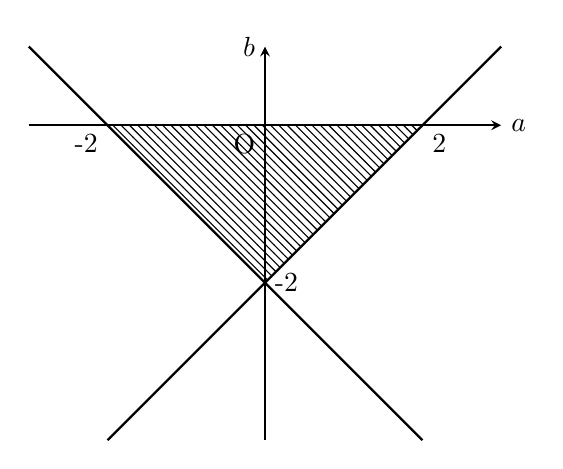
\begin{tikzpicture}[scale=1]
                    \draw[->, >=stealth, semithick] (-3,0)--(3,0) node[right]{$a$};
                    \draw[->, >=stealth, semithick] (0,-4)--(0,1) node[left]{$b$};
                    \draw[thick, domain=-3:2] plot(\x,-\x-2);
                    \draw[thick, domain=-2:3] plot(\x,\x-2);
                    \draw (0,0) node[below left]{O};
                    \draw (-2,0) node[below left]{-2};
                    \draw (2,0) node[below right]{2};
                    \draw (0,-2) node[right]{-2};
                    \fill [pattern = north west lines] (-2,0)--(2,0)--(0,-2);
               \end{tikzpicture}
               \caption{\cref{question:ut2021}の解答}
          \label{fig:pic0}
     \end{figure}

     条件$\phi(a,b)$のままでは図示できなかったことの要因は,条件$\phi(a,b)$に登場する変数が$a,b$だけでなく,
     量化記号$\exists$で束縛された変数$x_1, x_2$も登場していた事である.
     条件$\phi(a,b)$を満たす集合を図示するためには,その条件に同値な,
     量化記号$\exists$で束縛された変数のない条件$\theta(a,b)$を求める必要がある.

     このように,点$(a,b)$に関する条件$\phi(a,b)$から,それと同値な,
     量化記号で束縛された変数のない条件$\theta(a,b)$を求めることを,量化記号消去という.

     実数についての任意の条件は,量化記号消去ができるということは,
     Tarski \cite{MR0044472}によって示されていたが,
     Collins \cite{MR0403962}がより実用的な,柱状代数分解を用いたアルゴリズムを提案した.

     Collinsのアルゴリズムのアイデアを,次の問題を通して説明する.
     \todo[inline]{この辺まではいったん考えた}
     \begin{question}
          ある実数$x$が存在して
          $x^2 + a^2 < 1$, $a < x$
          を満たす実数$a$の範囲を求めよ.          
     \end{question}
     まず,$f(x,a) = x^2 + a^2 -1$, $g(x,a) = a-x$とする.
     この問題は,$a$についての条件
     \begin{equation}
          \phi(a) = \exists x (f(x,a)<0 \land g(x,a)<0)
     \end{equation}
     に同値な,量化記号$\exists$のない条件$\theta(a)$を求めることに同値である.

     まず,$(a, x)$座標平面上に,$2$つのグラフ$f(a,x)=0$, $g(a,x)=0$および領域$f(a,x)<0$, $g(a,x)<0$を描画してみよう.
     \begin{figure}[H]
          \centering
          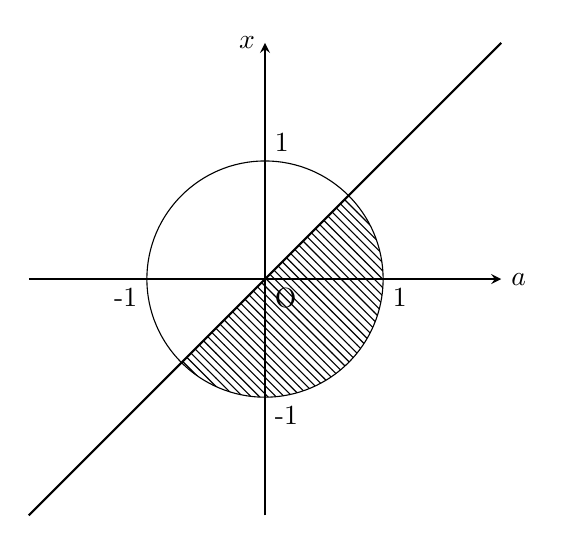
\begin{tikzpicture}[scale=1.5]
               \draw[->, >=stealth, semithick] (-2,0)--(2,0) node[right]{$a$};
               \draw[->, >=stealth, semithick] (0,-2)--(0,2) node[left]{$x$};
               \draw[thick, domain=-2:2] plot(\x,\x);
               \draw (0,0) circle(1 and 1);
               \draw (0,0) node[below right]{O};
               \draw (-1,0) node[below left]{-1};
               \draw (1,0) node[below right]{1};
               \draw (0,1) node[above right]{1};
               \draw (0,-1) node[below right]{-1};
               % \draw ({sqrt(1/2)},{sqrt(1/2)}) node[right]{$(1/\sqrt{2},1/\sqrt{2})$};
               % \draw ({-sqrt(1/2)},{-sqrt(1/2)}) node[left]{$(-1/\sqrt{2},-1/\sqrt{2})$};
               \begin{scope}
                    \clip (0,0) circle(1 and 1);
                    \fill[pattern = north west lines] (-2,-2)--(2,2)--(2,-2);
               \end{scope}
          \end{tikzpicture}          
          \caption{$f(x,a)=0, g(x,a)=0$のグラフの描画}
          \label{fig:pic1}
     \end{figure}
     
     ただし,領域$f(a,x)<0$, $g(a,x)<0$は図の斜線部分である.

     まず初めに,$f(a,x)$, $g(a,x)$の共有点と,それぞれの$a$方向の微分$\partial f/\partial a(a,x)$, $\partial g/\partial a(a,x)$ 
     が$0$になるような点$(-1,0)$, $(1,0)$, $(-1/\sqrt{2},-1/\sqrt{2})$, $(1/\sqrt{2},1/\sqrt{2})$を取る.

     \begin{figure}[H]
          \centering
          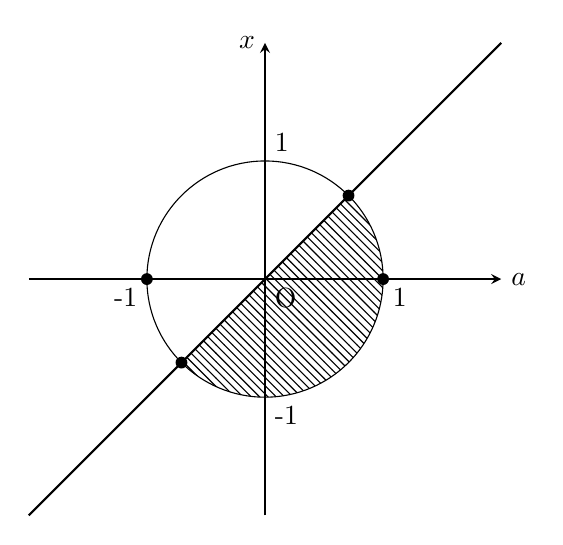
\begin{tikzpicture}[scale=1.5]
               \draw[->, >=stealth, semithick] (-2,0)--(2,0) node[right]{$a$};
               \draw[->, >=stealth, semithick] (0,-2)--(0,2) node[left]{$x$};
               \draw[thick, domain=-2:2] plot(\x,\x);
               \draw (0,0) circle(1 and 1);
               \draw (0,0) node[below right]{O};
               \draw (-1,0) node[below left]{-1};
               \draw (1,0) node[below right]{1};
               \draw (0,1) node[above right]{1};
               \draw (0,-1) node[below right]{-1};
               \fill (-1,0) circle(0.05 and 0.05);
               \fill (1,0) circle(0.05 and 0.05);
               \fill (-{sqrt(1/2)},-{sqrt(1/2)}) circle(0.05 and 0.05);
               \fill ({sqrt(1/2)},{sqrt(1/2)}) circle(0.05 and 0.05);
               \begin{scope}
                    \clip (0,0) circle(1 and 1);
                    \fill[pattern = north west lines] (-2,-2)--(2,2)--(2,-2);
               \end{scope}
          \end{tikzpicture}
          \caption{4点を描画}
          \label{fig:pic2}
     \end{figure}

     次に,この4点の$a$座標を境界にして,$a$軸を次のような開区間及び$1$点からなる$9$つの集合$\{S_i\}_{i=1}^9$に分割する.
     \begin{itemize}
          \item $S_1 \colon a < -1$,
          \item $S_2 \colon a = -1$,
          \item $S_3 \colon -1 < a < -1/\sqrt{2}$,
          \item $S_4 \colon a = -1/\sqrt{2}$,
          \item $S_5 \colon -1/\sqrt{2} < a < 1/\sqrt{2}$,
          \item $S_6 \colon a = 1/\sqrt{2}$,
          \item $S_7 \colon 1/\sqrt{2} < a < 1$,
          \item $S_8 \colon a = 1$,
          \item $S_9 \colon 1 < a$.
     \end{itemize}
     これらの条件を\cref{fig:pic2}に合わせて描画すると次のようになる.

     \begin{figure}[H]
          \centering
          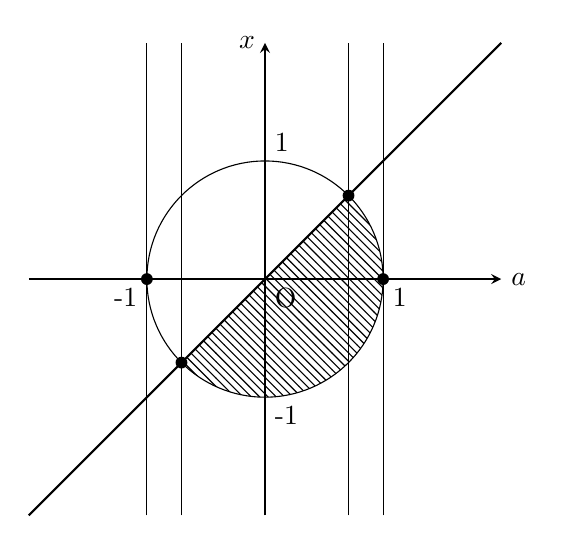
\begin{tikzpicture}[scale=1.5]
               \draw[->, >=stealth, semithick] (-2,0)--(2,0) node[right]{$a$};
               \draw[->, >=stealth, semithick] (0,-2)--(0,2) node[left]{$x$};
               \draw[thick, domain=-2:2] plot(\x,\x);
               \draw (0,0) circle(1 and 1);
               \draw (0,0) node[below right]{O};
               \draw (-1,0) node[below left]{-1};
               \draw (1,0) node[below right]{1};
               \draw (0,1) node[above right]{1};
               \draw (0,-1) node[below right]{-1};
               \draw (-1,-2)--(-1,2);
               \draw (-{sqrt(1/2)},-2)--(-{sqrt(1/2)},2);
               \draw ({sqrt(1/2)},-2)--({sqrt(1/2)},2);
               \draw (1,-2)--(1,2);
               \fill (-1,0) circle(0.05 and 0.05);
               \fill (1,0) circle(0.05 and 0.05);
               \fill (-{sqrt(1/2)},-{sqrt(1/2)}) circle(0.05 and 0.05);
               \fill ({sqrt(1/2)},{sqrt(1/2)}) circle(0.05 and 0.05);
               \begin{scope}
                    \clip (0,0) circle(1 and 1);
                    \fill[pattern = north west lines] (-2,-2)--(2,2)--(2,-2);
               \end{scope}
          \end{tikzpicture}

          \caption{$\{S_i\}_{i=1}^9$を描画}
          \label{fig:pic3}
     \end{figure}

     このような$a$軸の分割$\{S_i\}_{i=1}^9$をとると,
     各$S_i$に対し有限個の連続関数$\map{\xi_{S_i,1}, \cdots, \xi_{S_i,l_i}}{S_i}{\R}$を次を満たすようにとれる.
     \begin{itemize}
          \item 任意の$a \in S_i$に対し,$\xi_{S_i,1}(a) < \dots < \xi_{S_i,l_i}(a)$である.
          \item 任意の$a \in S_i$に対し,$\{\xi_{S_i,k}(a)\}_{j=1}^{l_i}$は$x$変数の多項式$f(a,x)$, $g(a,x)$の根全体である.
     \end{itemize}

     \todo{例}

     このとき各$S_i$に対し,$\xi_{S_i,0} \coloneqq -\infty$, $\xi_{S_i,l_i+1} \coloneqq \infty$として,
     \begin{align}
          C_{S_i, 2j} &= \{(a,\xi_{S_i, j}(a)) \in \R^2 \mid a \in S_i\}, \quad j=1,...,l_i,\\
          C_{S_i, 2j+1} &= \{(a,x) \in \R^2 \mid a \in S_i, \xi_{S_i,j}(a) < x < \xi_{S_i, j+1}(a)\}, \quad j=0,...,l_i,
     \end{align}
     と定めると,各$C_{S_i, k}$の上で$f, g$の符号は一定である.

     このようにして,$\R^2$の分割$\{C_{S_i,k}\}$を得ることができる.
     これを,$\R^2$の柱状代数分解という.厳密な定義は\cref{section:6}で行う.

     さて,
     \todo{推敲の余地}
     $a$についての条件$\phi(a)$に同値な量化記号のない条件$\theta(a)$を求めるには,
     ある$C_{S_i, k}$上で$f<0$, $g<0$となるような$S_i$を集めればよい.
     \cref{fig:pic3}より,そのような$S_i$全体は
     \begin{itemize}
          \item $S_5 \colon -1/\sqrt{2} < a < 1/\sqrt{2}$,
          \item $S_6 \colon a = 1/\sqrt{2}$,
          \item $S_7 \colon 1/\sqrt{2} < a < 1$
     \end{itemize}
     であるので,
     \begin{equation}
          \theta(a) \coloneqq (-1/\sqrt{2} < a < 1/\sqrt{2}) \land (a = 1/\sqrt{2}) \land (1/\sqrt{2} < a < 1)
     \end{equation}
     とすれば,これは論理式$\phi(a)$と同値な量化記号のない論理式である.

     上記の例のように,与えられた論理式$\phi(a)$に登場する多項式の集合${f,g}$から,
     ユークリッド空間の分割$\{S_i\}_{i=1}^9$, $\{C_{S_i,k}\}$を構成し,
     そこから適切な$S_i$を集め,それぞれの$S_i$を定める量化記号のない論理式の論理和をとることで,
     もとの論理式$\phi(a)$と同値な量化記号のない論理式$\theta(a)$を構成することができる.

     本論文では,このようなアルゴリズムを,実数体の代数的な性質を公理化した実閉体上で一般の論理式に対して行う.

     本論文は以下のように構成されている.% This paper is organized as follows:

     \cref{section:2}では,ArtinとSchreierにより導入された実閉体の概念についてまとめる.
     \cref{section:3}で一階述語論理の用語を導入し,さらに実閉体の理論を定義する.
     \cref{section:4}で理論が量化記号消去をもつことを定義し,実閉体の理論が量化記号消去を持つことを示す.
     
     そして,\cref{section:5}では,実閉体上の半代数的集合を定義し,その性質についてまとめる.この概念は,\cref{section:6}で定義する柱状代数分解に必要である.
     \cref{section:6}では,実閉体を係数とする多項式の有限部分集合$F$に対し,$F$適合な柱状代数分解について定義してその存在を示す.
     \cref{section:7}では,\cref{section:9}で述べる量化記号消去のアルゴリズムのために,\cref{section:6}の柱状代数分解を改良する.
     \cref{section:8}では,柱状代数分解と量化記号消去の関係について述べ,
     \cref{section:9}で述べるアルゴリズムが実際に任意の論理式の量化記号を消去する事を示す.
     最後に\cref{section:9}では,柱状代数分解による量化記号消去のアルゴリズムの疑似コードを明示する.

     \section*{謝辞}
     本修士論文の執筆にあたりたくさんの助言をくださった植田一石准教授に感謝の意を表します.

\section{実閉体}\label{section:2}

まず,\cite{MR3069467}でArtinとSchreierにより導入された,実閉体の概念についてまとめる.
始めに,順序体の定義を述べる.
以下の定義は\cite[Definition 1.1.1]{MR1659509}に従った.

\begin{definition}[順序体]
     体$F$と$F$上の全順序$<$の組$(F,<)$が次の性質を満たすとき,$(F,<)$を順序体(ordered field)という.
     \begin{enumerate}
          \item 任意の$x,y,z\in F$に対し,$x \leq y$ならば$x + z \leq y + z$である.
          \item 任意の$x,y \in F$に対し,$x \geq 0$, $y \geq 0$ならば$x \cdot y \geq 0$である.
     \end{enumerate}
\end{definition}

以下の定理が成り立つ.

\begin{theorem}[{cf.~\cite[Theorem 1.1.8]{MR1659509}}]\label{theorem:real-field}
     $F$を体とする.このとき,以下は同値である.
     \begin{enumerate}
          \item \label{theorem:real-field-1}
          $F$が順序体となるような全順序$<$を持つ.
          \item \label{theorem:real-field-2}
          任意の$x_1, \dots, x_n \in F$に対して
          \begin{equation}
               x_1^2 + \dots + x_n^2 \neq -1.
          \end{equation}
          \item \label{theorem:real-field-3}
          任意の$x_1, \dots, x_n \in F$に対して
          \begin{equation}
               \sum_{i=1}^n x_i^2 = 0 \Rightarrow x_1 = \dots = x_n = 0.
          \end{equation}
     \end{enumerate}
\end{theorem}

さらに,\cite[Definition 1.1.9]{MR1659509}に従い,実体を定義する.

\begin{definition}[実体]
     体$F$が\cref{theorem:real-field}の
     \ref{theorem:real-field-1},
     \ref{theorem:real-field-2},
     \ref{theorem:real-field-3}
     のいずれか(従って、全て)の条件を満たすとき,
     $F$を実体(real field)という.
\end{definition}


例えば,実数体$\R$や有理数体$\Q$,有理数体$\Q$に$\sqrt{2}$を添加した体$\Q\left(\sqrt{2}\right)$は,
通常の全順序構造を入れることにより順序体となる.
従って,$\R, \Q, \Q\left(\sqrt{2}\right)$はいずれも実体である.

また,複素数体$\C$は$\sqrt{-1}^2 = -1$を満たす元$\sqrt{-1}$を持つ.
従って,$\C$は実体ではない.

有理数体$\Q$は,実体$\Q\left(\sqrt{2}\right)$を代数拡大に持つが,
実数体$\R$の代数拡大で実体になるものは$\R$自身のみである.
そのような性質に注目し,実閉体の概念を導入する.

\begin{definition}[{\cite[Section I]{MR3069467}}] \label{definition:RCF}
     実体$F$が実閉体(real closed field)であるとは,
     $F$の代数拡大で実体になるものは$F$自身に限ることを指す.
\end{definition}

先ほど述べたように,有理数体$\Q$は実閉体ではないが,実数体$\R$は実閉体である.
また,代数的数全体(すなわち, 有理数体$\Q$の代数的閉包) $\overline{\Q}$と実数体$\R$の共通部分$\Ralg \coloneqq \overline{\Q} \cap \R$は実閉体である.
$\Ralg$の元を実代数的数という.

\begin{theorem}[{\cite[S\"{a}tze 1--3]{MR3069467}}] \label{theorem:real-closed-field}
     体$F$について,以下は同値である.
     \begin{enumerate}
          \item 体$F$は実閉体である.
          \item 次を満たす$F$の順序体の構造$<$がただ一つ存在する.
               \begin{itemize}
                    \item 任意の$x \in F$に対し, $x>0$ならば$x = y^2$を満たす$y \in F$が存在する.
                    \item 奇数次数の$F$係数$1$変数多項式は,$F$において少なくとも$1$つの根を持つ.
               \end{itemize}
          \item $F\left[\sqrt{-1}\right] \coloneqq F[X]/(X^2 + 1)$は代数的閉体である.
     \end{enumerate}
\end{theorem}

\cref{theorem:real-closed-field}の証明は,
\cite[Theorem 1.2.2]{MR1659509}を見よ.

以下では,実閉体$R$上の区間を,
\begin{equation}
     [a,b]\coloneqq\{x \in R \mid a \leq x \leq b\}, \quad (a,b)\coloneqq\{x \in R \mid a < x < b\}
\end{equation}
のようにかくことにする.

実閉体$R$を係数とする$1$変数多項式に対して,
実数体$\R$上の連続関数や可微分関数と同様の性質が成り立つ.

\begin{proposition}\label{proposition:intermediate}
     $R$を実閉体とし,$f \in R[X]$とする.
     任意の$a,b \in R$に対し,
     $a < b$かつ
     $f(a)f(b)<0$であれば,ある$x \in (a,b)$が存在して,$f(x)=0$を満たす.
\end{proposition}
\begin{proof}
     $R[\sqrt{-1}]$が代数的閉体であるから,
     $f(X)$の既約因子は,
     \begin{align}
          &X-\alpha, \\
          &(X-\beta)^2 + \gamma^2 = (X-\beta-\gamma\sqrt{-1})(X-\beta+\gamma\sqrt{-1})
     \end{align}
     の形のどちらかである($\alpha, \beta, \gamma \in R$, $\gamma \neq 0$).

     このとき,$(X-\beta)^2 + \gamma^2$の形の既約因子は,$\gamma \neq 0$としているから,$R$上で常に$0$より大きいことに注意する.
     $f(a)f(b)<0$であることから,$f(X)$のある既約因子$g(X)$について,$g(a)g(b)<0$となる.
     実際,もしすべての$f(X)$の既約因子$g(X)$について,$g(a)g(b) \geq 0$であれば,$f(a)f(b)\geq0$となり仮定に反する.
     ここで,先に述べた注意から,$g(a)g(b)<0$となるような$f(X)$の既約因子$g(X)$は,$g(X) = X - \alpha$とかける.
     $g(a)g(b) < 0$であることから,$a<\alpha<b$であり,このとき$f(\alpha)=0$である.
     従って,命題が示された.
\end{proof}

\begin{proposition}\label{proposition:Rolle}
     $R$を実閉体とし,$f \in R[X]$とする.
     任意の$a, b \in R$に対し,$a<b$かつ
     $f(a)=f(b)=0$であれば,ある$x \in (a,b)$が存在して,$f'(x)=0$である.
\end{proposition}
\begin{proof}
     $(a,b)$上に$f(X)$の根がない場合について示せば十分である.
     実際,もし$(a,b)$上に$f(X)$の根が存在するとき,それらの根を$a < x_1 < \dots < x_k < b$とすれば,
     $x_1$を改めて$b$とすることで$(a,b)$上に$f(X)$の根がない場合に帰着する.

     $(a,b)$上に$f(X)$の根がないと仮定し,
     \begin{equation}
     f(X) = (X-a)^m(X-b)^ng(X), \, g(a)\neq0,\, g(b)\neq0
     \end{equation}
     とおく.このとき,$(a,b)$上$g(X)$の根がないことから,\cref{proposition:intermediate}より,$g(a)g(b)>0$である.
     \begin{equation}
     g_1(X) \coloneqq m(X-b)g(X)+n(X-a)g(X)+(X-a)(X-b)g'(X)
     \end{equation}
     とおくと,
     \begin{equation}
          f'(X) = (X-a)^{m-1}(X-b)^{n-1}g_1(X)
     \end{equation}
     である.
     このとき,
     \begin{align}
     g_1(a) &= m(a-b)g(a), \\
     g_1(b) &= n(b-a)g(b)
     \end{align}
     であるから,$g_1(a)g_1(b)<0$である.
     よって,\cref{proposition:intermediate}より,ある$x \in (a, b)$が存在し$g_1(x)=0$である.
     この$x \in (a,b)$に対して$f'(x)=0$である.
\end{proof}

\begin{corollary}\label{corollary:mean-value}
     $R$を実閉体とし,$f \in R[X]$とする.
     任意の$a, b \in R$に対して,
     $a<b$であれば,
     ある$c \in (a,b)$が存在して,$f(b)-f(a) = (b-a)f'(c)$を満たす.
\end{corollary}

\begin{proof}
     $F(X) \in R[X]$を,
     \begin{equation}
          F(X) \coloneqq f(X) - \left\{\frac{f(b)-f(a)}{b-a}(X-a) + f(a)\right\}
     \end{equation}
     と定義すると,$F(a)=F(b)=0$であるから,\cref{proposition:Rolle}より,
     ある$c \in (a,b)$が存在して,$F'(c)=0$を満たす.
     この$c$に対して,$f(b)-f(a)=f'(c)(b-a)$が成り立つ.
\end{proof}

\begin{corollary}\label{corollary:monotone}
     $R$を実閉体とし,$f \in R[X]$とする.任意の$a, b \in R$に対して、$a<b$であれば以下が成り立つ.
     \begin{enumerate}
          \item \label{corollary:monotone-1}
          任意の$x \in (a,b)$に対して$f'(x)>0$ならば,$f(X)$は$[a,b]$上狭義単調増加である.
          \item \label{corollary:monotone-2}
          任意の$x \in (a,b)$に対して$f'(x)<0$ならば,$f(X)$は$[a,b]$上狭義単調減少である.
     \end{enumerate}
\end{corollary}
\begin{proof}
     \ref{corollary:monotone-2}は\ref{corollary:monotone-1}と同様に示せるので,\ref{corollary:monotone-1}のみ示す.
     $f(X)$が$[a,b]$上狭義単調増加でないとすると,ある$x \in (a,b)$に対して$f'(x) \leq 0$となることを示す.
     $f(X)$が$[a,b]$上狭義単調増加でないとすると,
     $a \leq x_0 < x_1 \leq b$である$x_0, x_1 \in R$が存在して,$f(x_0) \geq f(x_1)$を満たす.
     このとき,\cref{corollary:mean-value}より,$x_0 < x < x_1$である$x \in (a,b)$が存在して,
     $f(x_1) - f(x_0) = f'(x)(x_1 - x_0)$を満たすが、
     この$x \in (a,b)$に対して$f'(x) \leq 0$となる.
\end{proof}

\section{一階述語論理}\label{section:3}

この節では,\cite{MR1924282}に従って一階述語論理についてまとめる.

\begin{definition}[{\cite[Definition 1.1.1
     ]{MR1924282}}]
     以下のデータの組$\mathcal{L}$を言語(Language)という.
     \begin{enumerate}
          \item 関数記号(function symbol)の集合$\mathcal{F}$と,各$f \in \mathcal{F}$に対し正整数$n_f$を対応させる写像.
          \item 関係記号(relation symbol)の集合$\mathcal{R}$と,各$R \in \mathcal{R}$に対し正整数$n_R$を対応させる写像.
          \item 定数記号(constant symbol)の集合$\mathcal{C}$.
     \end{enumerate}
\end{definition}

ここで,$n_f$や$n_R$は,関数記号$f$と関係記号$R$がそれぞれ$n_f$変数,$n_R$変数を取ることを意味する.

次に,言語$\mathcal{L}$が与えられたときの構造について定義する.

\begin{definition}[{\cite[Definition 1.1.2]{MR1924282}}]
     以下のデータの組$\mathcal{M}$を$\mathcal{L}$構造($\mathcal{L}$-structure)という.
     \begin{enumerate}
          \item 空でない集合$M$. 
          \item 各$f \in \mathcal{F}$に対し,関数$\map{f^\mathcal{M}}{M^{n_f}}{M}$を対応させる写像.
          \item 各$R \in \mathcal{R}$に対し,集合$R^\mathcal{M} \subset M^{n_R}$を対応させる写像.
          \item 各$c \in \mathcal{C}$に対し,$c^\mathcal{M} \in M$を対応させる写像.
     \end{enumerate}
\end{definition}

$f^\mathcal{M}$, $R^\mathcal{M}$, $c^\mathcal{M}$を,
それぞれ$f \in \mathcal{F}$, $R \in \mathcal{R}$, $c \in \mathcal{C}$の解釈(interpretation)と呼ぶ,

次に,
言語$\mathcal{L}$の記号のほかに,
変数記号(variable symbol) $v_1, v_2, \dots$, 
等号(equality symbol) $=$,
論理記号(logic symbol) $\lor, \land, \lnot, \exists, \forall$
および括弧$($, $)$を用いて,項と論理式を定義する.

\begin{definition}[{\cite[Definition 1.1.4]{MR1924282}}]
     $\mathcal{L}$項($\mathcal{L}$-term)の集合とは,次を満たす最小の集合$\mathcal{T}$である.
     \begin{enumerate}
          \item 定数記号$c \in \mathcal{C}$に対し,$c \in \mathcal{T}$である.
          \item 変数記号$v_i$, $i=1, 2, \dots$, に対し,$v_i \in \mathcal{T}$である.
          \item 関数記号$f \in \mathcal{F}$および$t_1, \dots, t_{n_f} \in \mathcal{T}$に対し,$f(t_1, \dots, t_{n_f}) \in \mathcal{T}$である.
     \end{enumerate}
\end{definition}

$\mathcal{M}$を$\mathcal{L}$構造とする.$\mathcal{L}$項$t$が含む変数記号が高々$v_{i_1}, \dots, v_{i_m}$であるとする.
このとき,$t$を写像$\map{t^\mathcal{M}}{M^m}{M}$として解釈したい.
そこで,$\bar{a} = (a_{i_1}, \dots, a_{i_m}) \in M^m$に対し,$t^\mathcal{M}(\bar{a})$を,以下のように帰納的に定義する.

\begin{enumerate}
     \item 定数記号$c \in \mathcal{C}$に対し,$c^\mathcal{M}(\bar{a}) \coloneqq c^\mathcal{M}$とする.
     \item 変数記号$v_{i_j}$, $j=1, \dots, m$, に対し,$v_{i_j}(\bar{a}) \coloneqq a_{i_j}$とする.
     \item 
     関数記号$f \in \mathcal{F}$とする.
     さらに$t_1, \dots, t_{n_f}$を,文字列に含む変数記号が高々$v_{i_1}, \dots, v_{i_m}$である$\mathcal{L}$項で,
     それぞれ$t_i^\mathcal{M}(\bar{a})$が定義されているとする.
     このとき,$t = f(t_1, \dots, t_{n_f})$に対し,
     \begin{equation}
          t^\mathcal{M}(\bar{a})\coloneqq f^\mathcal{M}(t_1^\mathcal{M}(\bar{a}), \dots, t_{n_f}^\mathcal{M}(\bar{a}))
     \end{equation}
     と定義する.
\end{enumerate}

\begin{definition}[{\cite[Definition 1.1.5]{MR1924282}}]
     まず,$\mathcal{L}$原子論理式(atomic $\mathcal{L}$-formula)を,次のいずれかの形をした記号列として定義する.
     \begin{enumerate}
          \item $t_1, t_2$を$\mathcal{L}$項として,$(t_1 = t_2)$.
          \item $R \in \mathcal{R}$を述語記号,$t_1, \dots, t_{n_R}$を$\mathcal{L}$項として,$(R(t_1, \dots, t_{n_R}))$.
     \end{enumerate}
     次に,$\mathcal{L}$論理式($\mathcal{L}$-formula)の集合を,以下を満たす最小の集合$\mathcal{W}$として定義する.
     \begin{enumerate}
          \item $\mathcal{W}$は,全ての$\mathcal{L}原子論理式$を含む.
          \item $\phi \in \mathcal{W}$ならば,$\lnot \phi \in \mathcal{W}$である.
          \item $\phi, \psi \in \mathcal{W}$ならば,$(\phi \lor \psi), (\phi \land \psi) \in \mathcal{W}$である.
          \item $\phi \in \mathcal{W}$ならば,任意の変数記号$v_i$に対し$\forall v_i \phi, \exists v_i \phi \in \mathcal{W}$である.
     \end{enumerate}
\end{definition}

$\mathcal{L}$原子論理式およびその否定を,$\mathcal{L}$リテラル($\mathcal{L}$-literal)とよぶ.

ここで,論理式$\phi \coloneqq \forall x (x^2 + y > 0)$について観察する.ここで,$x,y$はいずれも変数記号である.
これは,「全ての$x$に対して$x^2 + y > 0$が成り立つ」というように読むことができるが,$y$の値は自由に設定することができ,$y$の値が定まらない限りは真であるか偽であるかははっきりしない.
この$y$のように,自由な状態にある変数記号を論理式$\phi$の自由変数という.
厳密には,次のように定義する.以下の定義は,\cite[定義 1.5.1]{C3041}を参考にした.

\begin{definition}
     $\mathcal{L}$を言語とする.
     $\mathcal{L}$項$t$に登場する全ての変数記号を$\Var(t)$で表す.
     $\mathcal{L}$論理式$\phi$の自由変数(free variable)全体$\Var(\phi)$を,次のように帰納的に定義する.
     \begin{enumerate}
          \item $t_1, t_2$を項とするとき,$\Var((t_1=t_2))\coloneqq\Var(t_1)\cup\Var(t_2)$と定義する.
          \item $R \in L$を$n$変数述語記号,$t_1, \dots, t_n$を項とするとき,$\Var(R(t_1, \dots, t_n))\coloneqq \bigcup_{i=1}^n \Var(t_i)$と定義する.
          \item 論理式$\phi$に対して$\Var(\phi)$が定義されているとき,$\Var(\lnot \phi)\coloneqq\Var(\phi)$と定義する.
          \item 論理式$\phi, \psi$に対して$\Var(\phi), \Var(\psi)$が定義されているとき,
          $\Var((\phi \lor \psi))\coloneqq\Var(\phi)\cup\Var(\psi)$,
          $\Var((\phi \land \psi))\coloneqq\Var(\phi)\cup\Var(\psi)$,
          と定義する.
          \item 論理式$\phi$に対して,$\Var(\phi)$が定義されているとき,変数記号$x$に対して
          $\Var(\forall x\phi)\coloneqq\Var(\phi) \setminus \{x\}$,
          $\Var(\exists x\phi)\coloneqq\Var(\phi) \setminus \{x\}$
          と定義する.
     \end{enumerate}
     自由変数でない変数を,束縛変数(bound variable)という.
     $\mathcal{L}$論理式$\phi$に登場する自由変数が高々$x_1, \dots, x_n$である事を明示したいとき,$\phi(x_1, \dots, x_n)$と書く.ただし,登場しない自由変数があっても良い.
     $\mathcal{L}$論理式$\phi$が自由変数を持たないとき,すなわち$\Var(\phi)=\emptyset$であるとき,
     $\phi$を$\mathcal{L}$文($\mathcal{L}$-sentense)という.
\end{definition}

\begin{definition}[{\cite[Definition 1.1.6]{MR1924282}}]
     $\mathcal{M}$を$\mathcal{L}$構造とする.
     $\mathcal{L}$論理式$\phi$が$\bar{v} = (v_{i_1}, \dots, v_{i_m})$を自由変数に持つとし,$\bar{a} = (a_{i_1}, \dots, a_{i_m}) \in M^m$とする.
     このとき,帰納的に$\mathcal{M} \models \phi(\bar{a})$を定義する.
     \begin{enumerate}
          \item 
               $\phi$が$(t_1=t_2)$である場合,
               $\mathcal{M} \models \phi(\bar{a})$を$t_1^\mathcal{M}(\bar{a}) = t_2^\mathcal{M}(\bar{a})$により定義する.
          \item 
               $\phi$が$(R(t_1, \dots, t_{n_R}))$である場合,
               $\mathcal{M} \models \phi(\bar{a})$を$(t_1^\mathcal{M}(\bar{a}), \dots, t_{n_R}^\mathcal{M}(\bar{a}))\in R^\mathcal{M}$により定義する.
          \item
               $\phi$が$\lnot \psi$である場合,
               $\mathcal{M} \models \phi(\bar{a})$を,$\mathcal{M} \models \psi(\bar{a})$でないことにより定義する.
          \item
               $\phi$が$(\psi \lor \theta)$である場合,
               $\mathcal{M} \models \phi(\bar{a})$を,
               $\mathcal{M} \models \psi(\bar{a})$または
               $\mathcal{M} \models \theta(\bar{a})$であることにより定義する.
          \item
               $\phi$が$(\psi \land \theta)$である場合,
               $\mathcal{M} \models \phi(\bar{a})$を,
               $\mathcal{M} \models \psi(\bar{a})$かつ
               $\mathcal{M} \models \theta(\bar{a})$であることにより定義する.
          \item
               $\phi$が$\exists v_j\psi(\bar{v}, v_j)$である場合,
               $\mathcal{M} \models \phi(\bar{a})$を,
               ある$b \in \mathcal{M}$が存在して
               $\mathcal{M} \models \psi(\bar{a},b)$であることにより定義する.
          \item
          $\phi$が$\forall v_j\psi(\bar{v}, v_j)$である場合,
          $\mathcal{M} \models \phi(\bar{a})$を,
          全ての$b \in \mathcal{M}$に対して
          $\mathcal{M} \models \psi(\bar{a},b)$であることにより定義する.
     \end{enumerate}
     $\mathcal{M} \models \phi(\bar{a})$であるとき,$\mathcal{L}$構造$\mathcal{M}$は$\phi(\bar{a})$を満たすという.
\end{definition}

\begin{remark}
     以下の点に注意する.

     \begin{itemize}
          \item
               論理式$\phi, \psi$に対し,
               $\phi \rightarrow \psi$を,$\lnot \phi \lor \psi$の省略とし,
               $\phi \leftrightarrow \psi$を,$(\phi \rightarrow \psi)\land(\psi \rightarrow \phi)$の省略とする.
               また,項$t_1, t_2$に対し,$t_1 \neq t_2$を,$\lnot(t_1 = t_2)$の省略とする.
          \item
               有限個の論理式$\phi_1, \dots, \phi_n$に対して,$\bigvee_{i=1}^n \phi_i$を$(\phi_1 \lor (\phi_2 \lor (\dots \lor \phi_n)))$の省略とする.
               また,$\bigwedge_{i=1}^n \phi_i$を$(\phi_1 \land (\phi_2 \land (\dots \land \phi_n)))$の省略とする.
          \item     
               変数記号は,$v_1, v_2, \dots, $に加え,他の記号$a, b, c, \dots, x, y, z, x_1, x_2, \dots$等も用いることにする.
          \end{itemize}
\end{remark}


\begin{definition}[{\cite[Section 1.2]{MR1924282}}]
     $\mathcal{L}$を言語とする.
     $\mathcal{L}$文からなる集合$T$を,$\mathcal{L}$理論($\mathcal{L}$-theory)という.
     さらに,$\mathcal{L}$構造$\mathcal{M}$が,任意の$\phi \in T$に対し
     $\mathcal{M} \models \phi$を満たすとき,$\mathcal{L}$構造$\mathcal{M}$を$\mathcal{L}$理論$T$のモデル(model)と言い,
     $\mathcal{M} \models T$とかく.
\end{definition}

ここで,実閉体の理論$\RCF$を,\cite[Section 5.2.1]{C3041}に従って定義する.

\begin{definition}[実閉体の理論]
     言語$\mathcal{L}_\mathrm{OR}$を,以下のデータの組として定義する.
     \begin{itemize}
          \item 定数記号 $0$, $1$.
          \item 1変数関数記号 $-$.
          \item 2変数関数記号 $+$, $\cdot$.
          \item 2変数関係記号 $<$.
     \end{itemize}
     更に,言語$\mathcal{L}_\mathrm{OR}$上の実閉体の理論$\RCF$を,
     以下の$\mathcal{L}_\mathrm{OR}$文全体からなる集合として定義する.
          \begin{enumerate}
               \item $\forall x \forall y \forall z(x + (y + z) = (x + y) + z)$,
               \item $\forall x (x + 0 = x)$,
               \item $\forall x ((x + (-x) = 0)\land((-x) + x = 0))$,
               \item $\forall x \forall y (x + y = y + x)$,
               \item $\forall x \forall y (x \cdot y = y \cdot x)$,
               \item $\forall x \forall y \forall z((x \cdot y) \cdot z = x \cdot (y \cdot z))$,
               \item $\forall x \forall y \forall z(x \cdot (y + z) = x \cdot y + x \cdot z)$,
               \item $\forall x (x \cdot 1 = x)$,
               \item $0 \neq 1$,
               \item $\forall x \exists y (x \neq 0 \rightarrow x \cdot y = 1)$,
               \item $\forall x \lnot (x < x)$,
               \item $\forall x \forall y \forall z(x < y \land y < z \rightarrow x < z)$,
               \item $\forall x \forall y (x < y \lor x = y \lor y < x)$,
               \item $\forall x \forall y \forall z(x < y \rightarrow x + z < y + z)$,
               \item $\forall x \forall y (0 < x \land 0 < y \rightarrow 0 < x \cdot y)$,
               \item $\forall x \exists y (x = y^2 \lor -x = y^2)$
               \item $\forall x_{2n} \dots \forall x_1 \forall x_0 \exists y (y^{2n+1} + x_{2n} \cdot y^{2n} + \cdots + x_1 \cdot y + x_0 = 0)$ ( $n =  1, 2 , \dots$ ).
          \end{enumerate}

     ここで,項$t$に対し,$t^p$は$t$の$p$個の積$(t\cdot(t\cdot(\dots \cdot t)))$の省略とする.
\end{definition}

\begin{remark}以下の点に注意する.
     \begin{itemize}
          \item 
          定数記号$1$の$p$個の和$(1+(1 + (\dots + 1)))$の省略として$p$を用いる.
          \item 
          $t \leq t'$を,$(t<t') \lor (t=t')$の省略とする.
          \item
          $t > t'$, $t \geq t'$を,それぞれ$t' < t$, $t' \leq t$の省略とする.
     \end{itemize}
\end{remark}


言語$\mathcal{L}_{\mathrm{OR}}$において,$\mathcal{L}_\mathrm{OR}$構造$\R=(\R,0,1,-,+,\cdot,<)$や$\Ralg=(\Ralg,0,1,-,+,\cdot,<)$は,
\begin{equation}
     \R \models \RCF, \quad \Ralg \models \RCF
\end{equation}
であり,構造$\R$,$\Ralg$はいずれも実閉体の理論$\RCF$のモデルである.

\begin{definition}[{\cite[Definition 1.2.12]{MR1924282}}]
     $T$を$\mathcal{L}$理論とし,$\phi$を$\mathcal{L}$文とする.
     $\phi$が$T$の論理的帰結(logical consequence)であるとは,任意の$T$のモデル$\mathcal{M}$に対し,
     $\mathcal{M} \models \phi$であることと定義する.
     $\phi$が$T$の論理的帰結であるとき,$T \models \phi$とかく.

     特に,$T = \emptyset$の場合,全ての$\mathcal{L}$構造は$T$のモデルである.$\phi$が$T=\emptyset$の論理的帰結であることを,
     $\models \phi$と表す.
\end{definition}

$\mathcal{L}$論理式$\phi$に現れる自由変数が高々$v_1, \dots, v_n$であるとする.
$T \models \forall v_1 \dots \forall v_n \phi(v_1, \dots, v_n)$が成り立つとき,
同様に$\mathcal{L}$論理式$\phi$は$\mathcal{L}$理論$T$の論理的帰結であるといい,$T \models \phi$と表す.

最後に,以下の3つの命題を示す.

\begin{proposition}\label{proposition:nnt}
     任意の$\mathcal{L}$論理式$\phi$に対し,
     $\mathcal{L}$リテラルから論理記号$\forall$, $\exists$, $\lor$, $\land$のみによって生成される$\mathcal{L}$論理式$\psi$が存在し,
     \begin{equation}
          \models \phi \leftrightarrow \psi
     \end{equation}
     である.このような$\mathcal{L}$論理式$\psi$を否定標準形(negation normal form)の論理式という.
\end{proposition}
\begin{proof}
     De Morganの法則
     \begin{align}
          &\models \lnot (\theta_1 \lor \theta_2) \leftrightarrow (\lnot \theta_1 \land \lnot \theta_2)\\
          &\models \lnot (\theta_1 \land \theta_2) \leftrightarrow (\lnot \theta_1 \lor \lnot \theta_2)
     \end{align}
     量化記号の否定
     \begin{align}
          &\models \lnot \forall x \theta \leftrightarrow \exists x \lnot \theta\\
          &\models \lnot \exists x \theta \leftrightarrow \forall x \lnot \theta
     \end{align}
     及び二重否定の除去
     \begin{equation}
          \models \lnot \lnot \theta \leftrightarrow \theta
     \end{equation}
     を用いて,否定記号$\lnot$を括弧の内側に入れていくことで示される.
\end{proof}

\begin{proposition}\label{proposition:dnf}
     任意の量化記号のない$\mathcal{L}$論理式$\phi$に対して,有限個の$\mathcal{L}$リテラル$L_{i,j}$が存在して
     \begin{equation}
          \models \phi \leftrightarrow \bigvee_{i=1}^n \bigwedge_{j=1}^{m_i} L_{i,j}
     \end{equation}
     を満たす.$\bigvee_{i=1}^n \bigwedge_{j=1}^{m_i} L_{i,j}$の形をした論理式を,和積標準形(disjunctive normal form)の論理式という.
\end{proposition}

\begin{proof}

     \cref{proposition:dnf}より,$\mathcal{L}$論理式$\phi$が否定標準形の論理式の場合に命題が成り立つことを示せばよい.
     この場合,$\phi$は量化記号のない論理式であるから,$\phi$に含まれる論理記号は$\lor$, $\land$のみであることに注意する.
     
     $\phi$に含まれる論理記号の数に関する帰納法で証明する.

     まず,$\phi$が原子論理式の場合は明らかである.

     次に,論理記号の数が$k$個以下である場合に命題が成り立つと仮定して,論理記号の数が$k+1$個の論理式$\phi$の場合にも命題が成り立つことを示す.
     このとき,$\phi = \psi \lor \psi'$または$\phi = \psi \land \psi'$とかける,
     帰納法の仮定より,
     \begin{align}
          &\models \psi \leftrightarrow \bigvee_{i} \bigwedge_j L_{i,j},\\
          &\models \psi' \leftrightarrow \bigvee_{i'} \bigwedge_{j'} L'_{i',j'}
     \end{align}
     であるように有限個のリテラル$L_{i,j}$および$L'_{i,j}$を取ることができる.
     このとき,
     \begin{align}
          &\models \psi \lor  \psi' \leftrightarrow \left( \bigvee_i \bigwedge_j L_{i,j} \right) \vee \left( \bigvee_{i'} \bigwedge_{j'} L'_{i',j'}\right)\\
          &\models \psi \land \psi' \leftrightarrow \bigvee_{i, i'} \left(\bigwedge_j L_{i,j} \wedge \bigwedge_{j'} L'_{i',j'}\right)
     \end{align}
     であるから,論理式$\phi$についても命題が成り立つ.
     従って,帰納法により命題が示された.
\end{proof}

\begin{proposition}\label{proposition:pnf}
     任意の$\mathcal{L}$論理式$\phi$に対し,ある量化記号のない$\mathcal{L}$論理式$\psi$及び量化記号$\Qua_1, \dots, \Qua_m \in \{\forall, \exists\}$が存在して,
     \begin{equation}
          \models \phi \leftrightarrow \Qua_1 v_1 \dots \Qua_m v_m \psi
     \end{equation}
     を満たす.$\Qua_1 v_1 \dots \Qua_m v_m \psi$の形をした論理式を冠頭標準形(prenex normal form)の論理式という.
\end{proposition}
\begin{proof}
     \cref{proposition:dnf}より,
     $\mathcal{L}$論理式$\phi$が否定標準形の論理式の場合に命題が成り立つことを示せばよい.
     
     $\phi$に含まれる論理記号の数に関する帰納法で証明する.
     
     まず,$\phi$が原子論理式の場合は明らかである.
     次に,論理記号の数が$k$個以下である場合に命題が成り立つと仮定して,論理記号の数が$k+1$個の論理式$\phi$の場合にも命題が成り立つことを示す.
     \begin{itemize}
          \item
               $\phi = \forall x \psi$または$\phi = \exists x \psi$の場合,
               帰納法の仮定より,ある量化記号のない論理式$\theta$および量化記号$\Qua_1, \dots, \Qua_m \in \{\forall, \exists\}$を用いて
               \begin{equation}
                    \models \psi \leftrightarrow \Qua_1 v_1, \dots, \Qua_m v_m \theta
               \end{equation}
               が成り立つ.よって,
               \begin{align}
                    &\models \forall x \psi  \leftrightarrow \forall x \Qua_1 v_1, \dots, \Qua_m v_m \theta\\
                    &\models \exists x \psi  \leftrightarrow \exists x \Qua_1 v_1, \dots, \Qua_m v_m \theta
               \end{align}
               より,論理式$\phi$についても命題が成り立つ.
          \item
               $\phi = \psi \land \psi'$または$\phi = \psi \lor \psi'$の場合,
               帰納法の仮定より,ある量化記号のない論理式$\theta, \theta'$および量化記号$\Qua_1, \dots, \Qua_m, \Qua'_1, \dots, \Qua'_{m'} \in \{\forall, \exists\}$を用いて
               \begin{align}
                    &\models \psi \leftrightarrow \Qua_1 v_1, \dots, \Qua_m v_m \theta\\
                    &\models \psi' \leftrightarrow \Qua'_1 w_1, \dots, \Qua'_{m'} w_{m'} \theta'
               \end{align}
               とできる.必要ならば変数記号を置き換えて,$\psi'$の自由変数に$v_1, \dots, v_m$が現れず,$\psi$の自由変数に$w_1, \dots, w_{m'}$が現れないとしてよい.
               このとき,
               \begin{align}
                    &\models \psi \land \psi' \leftrightarrow \Qua_1 v_1, \dots, \Qua_m v_m \Qua'_1 w_1, \dots, \Qua'_{m'} w_{m'}(\theta \land \theta')\\
                    &\models \psi \lor \psi' \leftrightarrow \Qua_1 v_1, \dots, \Qua_m v_m \Qua'_1 w_1, \dots, \Qua'_{m'} w_{m'}(\theta \lor \theta')
               \end{align}
               より,論理式$\phi$についても命題が成り立つ.
     \end{itemize}
     従って,帰納法により命題が示された.
\end{proof}


\section{量化記号消去}\label{section:4}

\begin{example} \label{example:quantifier elimination}
     言語$\mathcal{L}_\mathrm{OR}$上の次のような論理式を考える.
     \begin{equation} \label{eq:an example of a sentence with a quantifier}
          \phi(a) \coloneqq \forall x (x^2 + ax + a + 3 > 0)
     \end{equation}
     実閉体のモデルである実数体$\R$をとって考えると,
     論理式\eqref{eq:an example of a sentence with a quantifier}は
     次のように言い換えられる.
     \begin{equation}
          \text{任意の実数$x \in \R$に対して$x^2 + ax + a + 3 > 0$が成り立つ.}  
     \end{equation}
     これを変数記号$a$に対する条件と解釈すると,
     2次方程式$x^2 + ax + a + 3 = 0$の判別式
     $
     a^2 - 4 (a+3) = (a+2)(a-6)
     $
     が0より小さいことと同値であるから,
     \begin{equation}
          \theta(a) \coloneqq (-2 < a) \land (a < 6)
     \end{equation}
     に同値である.すなわち,次が成り立つ.
     \begin{equation}
          \R \models \forall a (\phi(a) \leftrightarrow \theta(a)).
     \end{equation}
\end{example}

\cref{example:quantifier elimination}において,
実は任意の$\RCF$のモデル$R$に対して
\begin{equation}
     R \models \forall a (\phi(a) \leftrightarrow \theta(a))
\end{equation}
が成り立つ.ここで,$\phi$には束縛変数$x$が現れており,一方で$\psi$に登場する変数記号は全て自由変数である.
つまり,$\phi$に登場する量化記号を消去し,自由変数のみの論理式$\psi$で記述できている.
このような現象を扱うために,「量化記号を消去する」という概念を定義する.


\begin{definition}[{\cite[Definition 3.1.1]{MR1924282}}]
$\mathcal{L}$理論$T$が量化記号消去(quantifier elimination)を持つとは,
任意の$\mathcal{L}$論理式$\phi$に対し,
量化記号のない論理式$\theta$が存在して,
\begin{equation}
     T \models \phi \leftrightarrow \theta
\end{equation}
が成り立つことを指す.
\end{definition}

\begin{theorem}[{\cite[Theorem 11]{MR0044472}}]\label{theorem:Tarski}
     言語$\mathcal{L}_\mathrm{OR}$上の実閉体の理論$\RCF$は量化記号消去を持つ.
\end{theorem}

これ以降,この節では\cref{theorem:Tarski}の証明を述べる.
$X_1, \dots, X_n$を変数記号とすると,
多項式
$
f(X_1, \dots, X_n) \in \Z[X_1, \dots, X_n]
$
は自然に$\mathcal{L}$項とみなせる.
原子論理式の表記法
\begin{align}
     \sign (f(X_1, \dots, X_n)) = 1 & \defiff f(X_1, \dots, X_n) > 0\\
     \sign (f(X_1, \dots, X_n)) = 0 & \defiff f(X_1, \dots, X_n) = 0\\
     \sign (f(X_1, \dots, X_n)) = -1 & \defiff f(X_1, \dots, X_n) < 0
\end{align}
を導入すると,
任意の原子論理式$\phi(X_1, \dots, X_n)$は,
ある多項式$f(X_1,\dots,X_n) \in \Z[X_1, \dots, X_n]$
及び$\sigma \in \{-1, 0, 1\}$を用いて
$\sign(f(X_1, \dots, X_n)) = \sigma$と書ける.
また,$\lnot(\sign(f(X_1, \dots, X_n)) = \sigma)$は,
$\bigvee_{\tau \in \{-1,0,1\} \setminus \{\sigma\}} (\sign(f(X_1, \dots, X_n)) = \tau)$
と同値である.

\begin{lemma}\label{lemma:qe_simplify}
     
     以下は同値である.
     \begin{enumerate}
          \item \label{lemma:qe_simplify_1}
          $\mathcal{L}_\mathrm{OR}$理論$\RCF$は量化記号消去を持つ.
          \item \label{lemma:qe_simplify_2}
          任意の正の整数$n$に対して,
          変数$Y_1, \dots, Y_n$をまとめて$\overline{Y}$と書くと,
          任意の正の整数$s$と
          任意の$f_1, \dots, f_s \in \Z \left[X, \overline{Y}\right]$
          および任意の写像$\map{\sigma}{\{1, \dots, s\}}{\{-1,0,1\}}$に対して,
          量化記号のない論理式$\theta\left(\overline{Y}\right)$が存在して,
          \begin{equation}
               \RCF \models \theta\left(\overline{Y}\right) \leftrightarrow \exists X \left(\bigwedge_{i=1}^s \left(\sign\left(f_i\left(X,\overline{Y}\right)\right) = \sigma(i)\right)\right)
          \end{equation}
          が成り立つ.
          \item \label{lemma:qe_simplify_3}
          任意の量化記号のない論理式$\phi\left(X, \overline{Y}\right)$に対し,
          ある量化記号のない論理式$\theta\left(\overline{Y}\right)$が存在して,
          \begin{equation}
               \RCF \models \theta\left(\overline{Y}\right) \leftrightarrow \exists X \phi\left(X, \overline{Y}\right)
          \end{equation}
          が成り立つ.
     \end{enumerate}
\end{lemma}

\begin{proof}
     \ref{lemma:qe_simplify_1}から\ref{lemma:qe_simplify_2}が従うことは明らかである.

     \ref{lemma:qe_simplify_2}から\ref{lemma:qe_simplify_3}が従うことを示す.
     \cref{proposition:dnf}から,%本来は\cref{propositon:dnf}を少しだけ改良したものである.
     任意の量化記号のない論理式$\phi(X, \overline{Y})$に対して,
     多項式$f_{i,j} \in \Z[X, \overline{Y}]$ ($i=1, \dots, k, j=1, \dots, l_i$)
     と$\map{\sigma_i}{\{1, \dots, l_i\}}{\{-1,0,1\}}$が存在して,
     \begin{equation}
          \RCF \models
          \phi\left(X, \overline{Y}\right) \leftrightarrow 
          \bigvee_{i=1}^k \bigwedge_{j=1}^{l_i} \left(\sign\left(f_{i,j}\left(X, \overline{Y}\right)\right) = \sigma_i(j)\right)
     \end{equation}
     が成り立つ.このとき,
     \begin{equation}
          \RCF \models 
          \exists X \phi\left(X, \overline{Y}\right) \leftrightarrow  
          \bigvee_{i=1}^k \left(\exists X \bigwedge_{j=1}^{l_i} \left(\sign\left(f_{i,j}\left(X, \overline{Y}\right)\right) = \sigma_i(j)\right)\right)
     \end{equation}
     が成り立つ.ここで,\ref{lemma:qe_simplify_2}より,
     各$i=1, \dots, k$に対して,
     \begin{equation}
          \RCF \models
          \theta_i\left(\overline{Y}\right) \leftrightarrow 
          \exists X \bigwedge_{j=1}^{l_i} \left(\sign\left(f_{i,j}\left(X, \overline{Y}\right)\right) = \sigma_i(j)\right)
     \end{equation}
     を満たす量化記号のない論理式$\theta_i\left(\overline{Y}\right)$が存在する.このとき,
     \begin{equation}
          \RCF \models
          \bigvee_i \theta_i\left(\overline{Y}\right)\leftrightarrow
          \exists X \phi\left(X, \overline{Y}\right) 
     \end{equation}
     である.従って,\ref{lemma:qe_simplify_3}が成り立つ.

     最後に,\ref{lemma:qe_simplify_3}から\ref{lemma:qe_simplify_1}が従うことを示す.
     \cref{proposition:pnf}より,任意の量化記号のない論理式$\phi\left(X_1, \dots, X_m, \overline{Y}\right)$および$\Qua_1, \dots, \Qua_m \in \{\forall, \exists\}$に対し,
     ある量化記号のない論理式$\theta\left(\overline{Y}\right)$が存在し,
     \begin{equation}
          \RCF \models 
          \Qua_1 X_1 \dots\Qua_m X_m \phi\left(X_1, \dots, X_m, \overline{Y}\right) \leftrightarrow \theta\left(\overline{Y}\right)
     \end{equation}
     を満たすことを示せばよい.これは,\ref{lemma:qe_simplify_3}と
     \begin{equation}
          \models \forall X \psi \leftrightarrow \lnot \exists X \lnot \psi
     \end{equation}
     を用いて,$m$に関する帰納法により示される.
     以上より,証明が完了した.
\end{proof}

\cref{lemma:qe_simplify}から,
\cref{theorem:Tarski}は次のように言い換えることができる.

\begin{theorem}[{\cite[Theorem 1.4.2]{MR1659509}}]\label{theorem:weak_Tarski}
     $\overline{Y} = (Y_1, \dots, Y_n)$と$X$を変数記号とする.任意の$f_1, \dots, f_s \in \Z\left[ \overline{Y},X \right]$および$\map{\sigma}{\{1, \dots, s\}}{\{-1, 0, 1\}}$に対して,
     量化記号のない論理式$\theta\left(\overline{Y}\right)$が存在して,次を満たす.

     任意の実閉体$R$と,任意の$\overline{y} = (y_1, \dots, y_n) \in R^n$に対し,次の2つが同値になる.
     \begin{enumerate}
          \item 実閉体$R$は$\exists X \bigwedge_{i=1}^s (\sign(f_i(X,\overline{y})) = \sigma(i))$ を満たす.
          \item 実閉体$R$は$\theta\left(\overline{y}\right)$を満たす.
     \end{enumerate}
\end{theorem}

\cref{theorem:weak_Tarski}により,次の系が成り立つ.
\begin{corollary}\label{corollary:weak_Tarski}
     $\overline{Y} = (Y_1, \dots, Y_n)$と$X$を変数記号とし,$R$を実閉体とする.
     任意の$f_1, \dots, f_s \in R\left[\overline{Y}, X\right]$及び$\map{\sigma}{\{1, \dots, s\}}{\{-1,0,1\}}$に対して,
     有限個の$g_{i,j} \in R\left[\overline{Y}\right]$及び$\tau_{i,j} \in \{-1, 0, 1\}$, $i=1, \dots, p, j=1, \dots, q_i$, が存在し,次を満たす.

     任意の$\overline{y} = (y_1, \dots, y_n) \in R^n$に対し,次の2つが同値になる.
     \begin{enumerate}
          \item ある$x \in R$が存在して,$\bigwedge_{i=1}^s (\sign_R(f_i(x, \overline{y})) = \sigma(i))$を満たす.
          \item $\bigvee_{i=1}^p \bigwedge_{j=1}^{q_i} (\sign_R(g_{i,j}(\overline{y})) = \tau_{i,j})$を満たす.
     \end{enumerate}
\end{corollary}

\begin{proof}
     自然数$m$と多項式$F_1, \dots, F_s \in R[X, \overline{Y}, \overline{T}]$を,次を満たすようにとれる.ただし,$\overline{T}$は変数記号$T_1, \dots, T_m$の列である.
     \begin{itemize}     
          \item   
               ある$\overline{a} \in R^m$が存在し,
               各$i=1, \dots, s$に対して$f_i(X,\overline{Y}) = F_i(X,\overline{Y}, \overline{a})$を満たす.
     \end{itemize}
     このとき,\cref{theorem:weak_Tarski}より,量化記号のない論理式$\theta(\overline{Y}, \overline{T})$を,次を満たすように取れる.

     任意の$(\overline{y}, \overline{t}) = (y_1, \dots, y_n, t_1, \dots, t_m) \in R^{n+m}$に対し,次の2つが同値になる.
     \begin{itemize}
          \item
               ある$x \in R$が存在して,$\bigwedge_{i=1}^s (\sign_R(F_i(x,\overline{y}, \overline{t})) = \sigma(i))$ を満たす.
          \item
               実閉体$R$は$\theta(\overline{y}, \overline{t})$を満たす.         
     \end{itemize}
     さらに,\cref{proposition:dnf}より,% 本来は\cref{proposition:dnf}を改良したものを使っている.
     多項式$G_{i,j} \in \Z[\overline{Y}, \overline{T}]$ と$\tau_{i,j}$, $i=1, \dots, p, j=1, \dots, q_i$, が存在して,
     \begin{equation}
          R \models
          \bigvee_{i=1}^p \bigwedge_{j=1}^{q_i}(\sign(G_{i,j}(\overline{Y}, \overline{T}))=\tau_{i,j})
          \leftrightarrow \theta(\overline{Y},\overline{T})
     \end{equation}
     を満たす.このとき,$g_{i,j}(\overline{Y}) \coloneqq G_{i,j}(\overline{Y}, \overline{a}) \in R[\overline{Y}]$とすればよい.
\end{proof}

これ以降,
この節では\cref{theorem:weak_Tarski}を\cite[Section 1.4]{MR1659509}に従って証明する.
まず,写像$\map{\sign_R}{R}{\{-1,0,1\}}$を
\begin{equation}
     \sign_R(a) \coloneqq
     \begin{cases}
          1 & a > 0 \\
          0 & a = 0 \\
          -1 & a < 0
     \end{cases}
\end{equation}
で定める.
多項式$f \in R[X]$に対し
\begin{align}
\ROOT(f) \coloneqq
\begin{cases}
     \{ x \in R \mid f(x) = 0 \} & f \ne 0, \\
     \emptyset & f = 0
\end{cases}
\end{align}
と置き,
有限個の多項式$f_1, \dots, f_s \in R[X]$に対し
\begin{align}
\ROOT(f_1,\ldots,f_s) \coloneqq \bigcup_{i=1}^s \ROOT(f_i)
\end{align}
の元を小さなものから順に並べて得られる列を
$(x_1,\dots,x_N)$と置く.
$m\coloneqq \max\{\deg(f_i) \mid i=1, \dots, s\}$と置くと,$N \leq sm$である.
また,$x_0 \coloneqq -\infty$,
$x_{N+1} \coloneqq \infty$とし,
各$k=0, \dots, N$に対し$I_k \coloneqq (x_k, x_{k+1})$と書く.
このとき,\cref{proposition:intermediate}より,
$x \in I_k$に対し$\sign_R(f(x))$は一定であるが,
これを$\sign_R(f_i(I_k))$と書く.
第$i$行が
\begin{equation}
     \sign_R(f_i(I_0)), \sign_R(f_i(x_1)), \sign_R(f_i(I_1)), \dots, \sign(f_i(x_N)), \sign(f_i(I_N))
\end{equation}
であるような$s$行$2N+1$列行列を$\SIGN_R(f_1, \dots, f_s)$と書く.
$\SIGN_R(f_1, \dots, f_s)$の各成分は$-1, 0, 1$のいずれかであることに注意する.
また,各成分が$-1,0,1$のいずれかである$s$行$(2l+1)$列行列
全体のなす集合の
$l \in \{0, 1, \ldots, sm\}$に関する和集合を
$W_{s,m}$と書く. 

\begin{lemma}[{\cite[Lemma 1.4.4]{MR1659509}}]\label{lemma:qe_1ststep}
     任意の正の整数$s, m$と,
     任意の写像$\map{\sigma}{\{1, \dots, s\}}{\{-1,0,1\}}$に対し,
     ある部分集合$W(\sigma) \subset W_{s,m}$が存在して,
     任意の実閉体$R$と,次数が$m$以下であるような任意の$f_1, \dots, f_s \in R[X]$に対し,以下が同値である.
     \begin{enumerate}
          \item $\SIGN_R(f_1, \dots, f_s) \in W(\sigma)$
          \item ある$x \in R$が存在して$\bigwedge_{i=1}^s (\sign_R(f_i(x)) = \sigma(i)$)が成り立つ.
     \end{enumerate}
\end{lemma}

\begin{proof}
     \begin{equation}
          W(\sigma)\coloneqq\{A \in W_{s,m} \mid \text{行列$A$のある列が$(\sigma(i))_{i=1}^s$である}\}
     \end{equation}
     とすればよい.
\end{proof}

次の補題は,\cref{theorem:weak_Tarski}の証明の中心となる補題である.

\begin{lemma}[{\cite[Lemma 1.4.5]{MR1659509}}]\label{lemma:qe_lowering}
     ある写像$\map{\varphi}{W_{2s,m}}{W_{s,m}}$が存在して,次を満たす.

     任意の実閉体$R$と,任意の$f_1, \dots, f_s \in R[X]$に対して,
     各$f_i$の次数は$m$以下であり,
     $f_s$は定数でなく,
     $f_1, \dots, f_{s-1}$はどれも恒等的に$0$ではないとする.
     このとき,$g_1, \dots, g_s \in R[X]$を,それぞれ$f_s$を$f_1, \dots, f_{s-1}$, $f_s'$で割った余りとすれば,
     \begin{equation}
          \SIGN_R(f_1, \dots, f_s) = \varphi(\SIGN_R(f_1, \dots, f_{s-1}, f_s', g_1, \dots, g_s))
     \end{equation}
     である.
\end{lemma}

この補題によって、
$\SIGN_R(f_1, \dots, f_s)$は
より易しい
$
\SIGN_R(f_1, \dots, f_{s-1}, f_s', g_1, \dots, g_s)
$
のみで決まる。

\begin{proof}
     $\ROOT(f_1, \dots, f_{s-1}, f'_s, g_1, \dots, g_s)$
     の元を小さいものから順に並べて得られる列を
     $(x_1, \dots, x_N)$と置き、
     $\ROOT(f_1,\ldots, f_{s-1}, f'_s)$
     の元をちいさいものから順に並べて得られる部分列を
     $(x_{i_1}, \dots, x_{i_M})$と置く.
     $N \leq 2sm$であることに注意せよ.
     数列$(i_i, \dots, i_M)$は
     行列
     $
     w \coloneqq
     \SIGN_R(f_1, \dots, f_{s-1}, f_s', g_1, \dots, g_s)
     $
     のみで決まる.
     $i_0\coloneqq 0$, $i_{M+1}\coloneqq N+1$, $x_0\coloneqq -\infty$, $x_{N+1}\coloneqq \infty$と置く.
     任意の$k \in \{1, \dots, M \}$に対し,
     $f_1, \dots, f_{s-1}, f_s'$のいずれかは$x_{i_k}$において$0$になる.
     従って,$\map{\theta}{\{1,\dots, M\}}{\{1, \dots, s\}}$を,次を満たすようにとれる.
     \begin{itemize}
          \item 各$k=1, \dots, M$に対して,$\theta(k) \in \{1, \dots, s-1\}$ならば$f_{\theta(k)}(x_{i_k})=0$
          \item 各$k=1, \dots, M$に対して,$\theta(k)=s$ならば$f_s'(x_{i_k}) = 0$
     \end{itemize}
     この性質を満たす$\theta$は,行列$w$の情報のみを用いて定義できることに注意する.
     また,この$\theta$に対して,各$k=1, \dots, M$において$f_s(x_{i_k}) = g_{\theta(k)}(x_{i_k})$が成り立つことにも注意する.

     さらに各$k=0, \dots, M$において,$f_s'$は区間$(x_{i_k}, x_{i_{k+1}})$の上で$0$でない一定の符号をもつから,\cref{corollary:monotone}より,
     $f_s$は区間$(x_{i_k}, x_{i_{k+1}})$上に高々一つの根を持つ.
     また,$f_s$が根を持つ必要十分条件は次のように述べられる.
     \begin{itemize}
          \item $M\neq0$の場合,$k=1, \dots, M-1$に対して,$f_s(X)$が区間$(x_{i_k}, x_{i_{k+1}})$上に解を持つことの必要十分条件は
          \begin{equation}
               \sign_R(g_\theta(k)(x_{i_k}))\sign_R(g_\theta(k+1)(x_{i_{k+1}})) = -1.
          \end{equation}
          \item $M\neq0$の場合,$(-\infty, x_1)$に解を持つことの必要条件は,
          \begin{equation}
               \sign_R(f_s'((-\infty, x_1))) \sign_R(g_\theta(1)(x_1)) = 1.
          \end{equation}
          \item $M\neq0$の場合,$(x_M, \infty)$に解を持つことの必要条件は,
          \begin{equation}
               \sign_R(f_s'((x_M, \infty))) \sign_R(g_\theta(M)(x_M)) = -1.
          \end{equation}
          \item $M = 0$の場合は,$(\infty, \infty)$上に必ず解を持つ.
     \end{itemize}
     いずれの条件も,行列$w$の情報のみで記述されることに注意する.

     さて,ここで$y_1 < \dots < y_L$ ($L \leq sm$) を
     $f_1, \dots, f_{s-1}, f_s$の$R$上の根全体とし,$y_0 = -\infty$, $y_{L+1} = \infty$とする.
     $\map{\rho}{\{0, \dots, L+1\}}{\{0, \dots, M+1\} \cup \{(k,k+1) \mid k=0, \dots, M\}}$を,
     \begin{equation}
          \rho(l) \coloneqq \begin{cases} 
               k & y_l = x_{i_k},\\
               (k, k+1) & y_l \in (x_{i_k}, x_{i_{k+1}})
          \end{cases}
     \end{equation}
     と定める.上記で述べたことより,$\rho$の定義は,行列$w$の情報にのみ依存する.

     それでは,$\SIGN_R(f_1, \dots, f_s)$が$w$の情報のみに依存して定まる事を示す.
     
     まず,$j=1, \dots, s-1$に対しては,
     \begin{equation}
          \sign_R(f_j(y_l)) = \begin{cases}
               \sign_R(f_j(x_{i_k})) & \rho(l) = k,\\
               \sign_R(f_j((x_{i_k}, x_{i_{k+1}}))) & \rho(l) = (k, k+1)
          \end{cases}
     \end{equation}
     であり,また,
     \begin{equation}
          \sign_R(f_j((y_l,y_{l+1}))) = \sign_R(f_j((x_{i_k}, x_{i_{k+1}}))) \quad \text{$\rho(l)=k$または$\rho(l)=(k,k+1)$}
     \end{equation}
     である.さらに,$j=s$に対しては,
     \begin{equation}
          \sign_R(f_s(y_l)) = \begin{cases}
               \sign_R(g_{\theta(k)}(x_{i_k})) & \rho(l) = k,\\
               0 & \rho(l) = (k, k+1)
          \end{cases}
     \end{equation}
     であり,また,
     \begin{equation}
          \sign_R(f_s((y_l,y_{l+1}))) = \begin{cases}
               \sign_R(g_{\theta(k)}(x_{i_k})) & \rho(l) = k, l \neq 0, g_{\theta(k)}(x_{i_k})\neq 0\\
               \sign_R(f_s'((x_{i_k},x_{i_{k+1}}))) & \rho(l)=k, l \neq 0, g_{\theta(k)}(x_{i_k}) = 0 \\
               \sign_R(f_s'((x_{i_k}, x_{i_{k+1}}))) & \rho(l) = (k, k+1), l \neq 0\\
               -\sign_R(f_s'((-\infty, x_1))) & l=0
          \end{cases}
     \end{equation}
     である.

     以上により$\SIGN_R(f_1, \dots, f_s)$は$w$の情報のみに依存して定まる.よって,証明が完了した.
\end{proof}

以上の準備をもとに,\cref{theorem:weak_Tarski}を示す.
\cref{lemma:qe_1ststep}により,\cref{theorem:weak_Tarski}の証明は,次の命題から従う.

\begin{proposition}[{\cite[Proposition 1.4.6]{MR1659509}}] \label{proposition:weak_Tarski}
     $\overline{Y}\coloneqq (Y_1, \dots, Y_n)$とし,
     $f_1, \dots, f_s \in \Z\left[X, \overline{Y}\right]$をそれぞれ
     $f_i \left(X, \overline{Y} \right) = h_{i, m_i}\left( \overline{Y} \right) X^{m_i} + \dots + h_{i, 0}\left(\overline{Y}\right)$ ($i=1, \dots, s$)とする.
     また,$m\coloneqq \max\{m_i \mid i=1, \dots, m\}$とする.
     任意の$W \subset W_{s,m}$に対し,
     ある量化記号のない論理式$\theta\left(\overline{Y}\right)$が存在して次を満たす.

     任意の実閉体$R$と,任意の$\overline{y} \coloneqq (y_1, \dots, y_n) \in R^n$に対し,以下の2つが同値である.
     \begin{enumerate}
          \item $\SIGN_R(f_1(X, \overline{y}), \dots, f_s(X, \overline{y})) \in W$である.
          \item 実閉体$R$は$\theta(\overline{y})$を満たす.
     \end{enumerate}
\end{proposition}

実際,\cref{proposition:weak_Tarski}において$W=W(\sigma)$とすれば,\cref{theorem:weak_Tarski}が従う.

\begin{proof}[\cref{proposition:weak_Tarski}の証明]
     一般性を失わずに,各多項式$f_i$は恒等的に$0$でなく,$h_{i, m_i} \neq 0$としてよい.
     ここで,多項式の列$(f_1, \dots, f_s)$に対して,各多項式の$X$についての次数の列$(m_1, \dots, m_s)$を対応づける.
     非負整数列全体$\{(m_1, \dots, m_s) \mid s \geq 1, m_1, \dots, m_s\}$上の前順序関係
     \begin{equation}
          (m_1, \dots, m_s) \prec (m_1', \dots, m_{s'}')
     \end{equation}
     を,ある非負整数$p$が存在し,以下の2条件を満たすことと定義する.
     \begin{itemize}
          \item $p$に等しい$m_i$ ($i=1, \dots, s$)の数が,$p$に等しい$m'_i$ ($i=1, \dots, s'$)の数より少ない.
          \item 任意の$q>p$に対して,$q$に等しい$m_i$ ($i=1, \dots, s$)の数が,$q$に等しい$m'_i$ ($i=1, \dots, s'$)の数より少ない.
     \end{itemize}
     この前順序関係$\prec$は,非負整数列全体の中に無限降鎖列は存在しない.
     すなわち,非負整数列の列$\{\mu_i\}_{i \geq 1}$で,$\mu_1 \succ \mu_2 \succ \dots$となるものは存在しない.
     この前順序関係$\prec$に関する帰納法を用いて,命題を証明をする.

     $m\coloneqq \max\{m_1, \dots, m_s\}$とする.$m=0$の場合,すなわち$f_1, \dots, f_s \in \Z\left[\overline{Y}\right]$の場合,
     $W'\coloneqq\{(a_i)_{i=1}^s \in W \mid \text{$(a_i)_{i=1}^s$は$s$行$1$列の行列}\}$として
     \begin{equation}
          \theta\left(\overline{Y}\right) \coloneqq \bigvee_{(a_i)_{i=1}^s \in W'}\bigwedge_{i=1}^s \left(\sign\left(f_i\left(\overline{Y}\right)\right)=a_i\right)
     \end{equation}
     とすれば,命題を満たす.

     次に,$m \geq 1$の場合を考える.
     この場合は,次数を下げていき,最終的に$f_1, \dots, f_s \in \Z\left[\overline{Y}\right]$の場合に帰着させることで示される.

     まず,多項式の順番を並び替えて,$m_s=m$であるとしてよい.
     \cref{lemma:qe_lowering}で示した$\map{\varphi}{W_{2s,m}}{W_{s,m}}$を取り,
     $W''\coloneqq \varphi^{-1}(W)$とする.
     \cref{lemma:qe_lowering}より,任意の実閉体$R$と,任意の$\overline{y} = (y_1, \dots, y_s) \in R^n$に対し,
     各$i=1, \dots, s$に対して$h_{i, m_i}(\overline{y}) \neq 0$であれば以下の2条件は同値である.
     \begin{itemize}
          \item $\SIGN_R(f_1(X,\overline{y}), \dots, f_s(X, \overline{y})) \in W$,
          \item $\SIGN_R(f_1(X,\overline{y}), \dots, f_{s-1}(X, \overline{y}), f_s'(X, \overline{y}), g_1(X,y), \dots, g_s(X,y)) \in W''$,
     \end{itemize}
     ここで,$g_1, \dots, g_{s-1}$は,それぞれ$f_s$を$f_1, \dots, f_{s-1}$により$X$に関して割った余りに,
     $h_{1, m_1}, \dots, h_{s-1, m_{s-1}}$の適切な偶数べき乗を,それぞれの分母が消去できるようにかけて得られる多項式である.
     また,$g_s$は,$f_s$を$f_s'$により$X$に関して割った余りに,$m_s h_{s,m_s}$の適切な偶数べき乗を,分母が消去できるようにかけて得られる多項式である.
     このとき,多項式列$f_1, \dots, f_{s-1}, f_s', g_1, \dots, g_s$の$X$についての次数は,前順序関係$\prec$に関して$(m_1, \dots, m_s)$よりも小さくなる.
 
     一方,ある$i=1, \dots, s$について$h_{i, m_i}(\overline{y}) = 0$である場合,
     そのような$i$については$\widetilde{f}_i \coloneqq f_i - h_{i, m_i}X^{m_i}$とし,
     それ以外の$i$については$\widetilde{f}_i \coloneqq f_i$として得られる多項式列$(\widetilde{f}_1, \dots, \widetilde{f}_s)$
     について,以下の2条件は同値である.
     \begin{itemize}
          \item $\SIGN_R(f_1(X,\overline{y}), \dots, f_s(X, \overline{y})) \in W$,
          \item $\SIGN_R(\widetilde{f}_1(X,\overline{y}), \dots, \widetilde{f}_s(X, \overline{y})) \in W$,
     \end{itemize}
     これにより,多項式列$\widetilde{f}_1, \dots, \widetilde{f}_s$の$X$についての次数が,前順序関係$\prec$に関して$(m_1, \dots, m_s)$よりも小さくなる.

     以上により命題の証明が完了した.
\end{proof}

\section{半代数的集合}\label{section:5}
\begin{definition}[{\cite[Definition 2.1.4]{MR1659509}}]
     $R$を実閉体とする.
     変数記号の列$X_1, \dots, X_n$を$\overline{X}$と書くことにする.
     集合$S \subset R^n$が有限個の$f_{i,j} \in R\left[\overline{X}\right]$
     および$\sigma_{i,j} \in \{-1, 0 ,1\}$, $i=1, \dots, s, j = 1, \dots, l_i$, をもちいて,
     \begin{align}
          S &= \bigcup_{i=1}^s \bigcap_{j=1}^{l_i} \{\overline{x} \in R^n \mid \sign_R(f_{i,j}(\overline{x})) = \sigma_{i,j}\}\\
            &= \left\{ \overline{x} \in R^n \middle| \bigvee_{i=1}^s \bigwedge_{j=1}^{l_i} \sign_R(f_{i,j}(\overline{x})) = \sigma_{i,j} \right\}
     \end{align}
     と書けるとき,$S$を$R^n$の半代数的部分集合(semi-algebraic subset), あるい単に半代数的集合(semi-algebraic set)という.
\end{definition}

さらに,半代数的集合の位相を定義する.

$x \in R^n$, $r \in R$, $r>0$に対して,
\begin{align}
     \norm{x} &\coloneqq \sqrt{x_1^2 + \dots + x_n^2},\\
     B_n(x,r) &\coloneqq \{y \in R^n \mid \norm{y-x} < r\}
\end{align}
と定義する.

このとき,$\{B_n(x,r)\}$を開基として$R^n$に位相を定義できる.
以降では,$R^n$にはこの位相が入っているものとする.

定義より,$R^n$の半代数的部分集合$S$は,量化記号のない$\mathcal{L}_\mathrm{OR}$論理式$\theta\left( \overline{X}, \overline{T} \right)$ 
(ただし,$\overline{T}$は変数記号の列$T_1, \dots, T_k$を表す)と$\overline{t} = (t_1, \dots, t_k) \in R^k$を用いて
\begin{equation}
     S = \left\{ \overline{x} \in R^n \middle| R \models \theta(\overline{x}, \overline{t}) \right\}
\end{equation}
と表すことができる.これは逆も成り立つ.

\begin{proposition} \label{proposition:semi-algebraic-set}
     $R$を実閉体とする.
     任意の量化記号のない$\mathcal{L}_\mathrm{OR}$論理式$\theta\left( \overline{X}, \overline{T} \right)$
     及び任意の$\overline{t} \in R^k$について,
     \begin{equation}
          S = \left\{ \overline{x} \in R^n \middle| R \models \theta(\overline{x}, \overline{t}) \right\}
     \end{equation}
     により定まる集合$S$は$R^n$の半代数的部分集合である.
\end{proposition}

\begin{proof}
     \cref{proposition:dnf}より,ある有限個の$F_{i,j} \in \Z\left[\overline{X}, \overline{T}\right]$および$\sigma_{i,j} \in \{-1, 0 ,1\}$, $i=1, \dots, s, j = 1, \dots, l_i$, が存在して,
     \begin{equation}
          R \models
          \bigvee_{i=1}^s \bigwedge_{j=1}^{l_i}(\sign(F_{i,j}(\overline{Y}, \overline{T}))=\sigma_{i,j})
          \leftrightarrow \theta(\overline{Y},\overline{T})
     \end{equation}
     が成り立つので,
     \begin{align}
          S &= \left\{ \overline{x} \in R^n \middle| R \models \bigvee_{i=1}^s \bigwedge_{j=1}^{l_i} \sign(F_{i,j}(\overline{x}, \overline{t})) = \sigma_{i,j} \right\}\\
            &= \left\{ \overline{x} \in R^n \middle| \bigvee_{i=1}^s \bigwedge_{j=1}^{l_i} \sign_R(F_{i,j}(\overline{x}, \overline{t})) = \sigma_{i,j} \right\}
     \end{align}
     である.これより命題が示された.
\end{proof}


\begin{remark}
     以下の点に注意する.
     \begin{itemize}
          \item 
               $S \subset R^n$が半代数的集合ならば,$R^n \setminus S$も半代数的集合である.
          \item 
               $S_1, S_2 \subset R^n$が半代数的集合ならば,$S_1 \cup S_2$, $S_1 \cap S_2$も半代数的集合である.
     \end{itemize}
\end{remark}

半代数的集合は,集合の合併,交叉,補集合を取る操作で閉じている.
さらに,射影を取る操作でも閉じている.すなわち,次の定理が成り立つ.

\begin{theorem}[{\cite[Theorem 2.2.1]{MR1659509}}]\label{theorem:Tarski-Seidenberg}
     $R$を実閉体とし,$S \subset R^{n+1}$を半代数的集合とする.$\map{\pi_{n}}{R^{n+1}}{R^n}$を,
     $\pi_{n}(x_1, \dots, x_n, x_{n+1}) = (x_1, \dots, x_n)$により定める.このとき,
     $\pi_{n}(S)$は$R^n$の半代数的部分集合である.
\end{theorem}

この定理は,次の命題から従う.

\begin{proposition} \label{proposition:Seidenberg-Tarski-generalization}
     $R$を実閉体とし,$\phi\left(\overline{X}, \overline{T}\right)$を$\mathcal{L}_\mathrm{OR}$論理式とする.
     また,$\overline{t} = (t_1, \dots, t_k) \in R^k$とする.
     このとき,
     \begin{equation}
          S = \left\{\overline{x} \in R^n \middle| R \models \phi\left(\overline{x},\overline{t}\right) \right\}
     \end{equation}
     により定まる集合$S$は,$R^n$の半代数的部分集合である.
\end{proposition}

\begin{proof}
     \cref{theorem:Tarski}より,ある量化記号のない$\mathcal{L}_\mathrm{OR}$論理式$\theta\left(\overline{X}, \overline{T}\right)$が存在し,
     \begin{equation}
          R \models \phi\left(\overline{X},\overline{T}\right) \leftrightarrow \theta\left(\overline{X}, \overline{T}\right)
     \end{equation}
     が成り立つ.従って,
     \begin{equation}
          S = \left\{ \overline{x} \in R^n \middle| R \models \theta(\overline{x}, \overline{t}) \right\}
     \end{equation}
     となり,\cref{proposition:semi-algebraic-set}より命題が示された.
\end{proof}

\begin{proof}[\cref{theorem:Tarski-Seidenberg}の証明]
     半代数的集合$S \subset R^{n+1}$は,
     ある量化記号のない$\mathcal{L}_\mathrm{OR}$論理式$\theta\left(\overline{X}, \overline{T}\right)$および$\overline{t} \in R^k$を用いて,
     \begin{equation}
          S = \left\{(x_1, \dots, x_n, x_{n+1}) \in R^{n+1} \middle| R \models \theta\left(x_1, \dots, x_n, x_{n+1}, \overline{t}\right)\right\}
     \end{equation}
     と表すことができる.このとき,
     \begin{align}
          \pi_n(S) = \left\{(x_1, \dots, x_n) \in R^n \middle|  R \models \exists X_{n+1} \theta\left(x_1, \dots, x_n, X_{n+1}, \overline{t}\right)\right\}
     \end{align}
     であるから,\cref{proposition:Seidenberg-Tarski-generalization}より,定理の主張が従う.
\end{proof}

\begin{proposition}\label{proposition:Artin-Lang}
     $R_1$, $R_2$を任意の実閉体とする.
     $\phi(X_1, \dots, X_n)$を$\mathcal{L}_\mathrm{OR}$論理式とする.
     このとき,
     \begin{equation}
          \{x \in R_1^n \mid R_1 \models \phi(x)\} \neq \emptyset \iff
          \{x \in R_2^n \mid R_2 \models \phi(x)\} \neq \emptyset
     \end{equation}
     が成り立つ.
\end{proposition}
\begin{proof}
     ある$x \in R_1^n$について$R_1 \models \phi(x)$が成り立つことと,
     \begin{equation}
          R_1 \models \exists X_1 \dots \exists X_n \phi(X_1, \dots, X_n)
     \end{equation}
     が成り立つことは同値.
     従って,\cref{theorem:Tarski}より,量化記号のない$\mathcal{L}_\mathrm{OR}$論理式$\theta$が存在し,
     $\theta$は自由変数を持たず,
     \begin{equation}
          \RCF \models \exists X_1 \dots \exists X_n \phi(X_1, \dots, X_n) \leftrightarrow \theta
     \end{equation}
     であるようにできる.
     また,\cref{proposition:dnf}より,$\mathcal{L}_\mathrm{OR}$論理式$\theta$は,
     有限個の$n_{i,j} \in \Z$及び$\sigma_{i,j} \in \{-1, 0, 1\}$を
     \begin{equation}
          \RCF \models \theta \leftrightarrow \bigvee_{i=1}^s \bigwedge_{j=1}^{l_i} (\sign(n_{i,j}) = \sigma_{i,j})
     \end{equation}
     が成り立つように取れる.
     これより,$\RCF \models \theta$であるか,$\RCF \models \lnot \theta$のいずれかを満たす.
     従って,$R_1 \models \theta \iff R_2 \models \theta$である. 
     よって,$\{x \in R_1^n \mid R_1 \models \phi(x)\} \neq \emptyset \iff \{x \in R_1^n \mid R_2 \models \phi(x)\} \neq \emptyset$である.
\end{proof}

\begin{definition}[{\cite[Definition 2.2.5]{MR1659509}}]
     $S \subset R^m$, $T \subset R^n$を,半代数的集合とする.
     写像$\map{f}{S}{T}$が半代数的(semi-algebraic)であるとは,$f$のグラフ
     \begin{equation}
          \Graph(f) = \{(x, y) \in R^m \times R^n \mid x \in A, f(x) = y\}
     \end{equation}
     が$R^{m+n}$の半代数的部分集合であることを指す.
\end{definition}

このとき,次の命題が成り立つ.

\begin{proposition}\label{proposition:image-preimage}
     $\map{f}{A}{B}$を,半代数的写像であるとする.
     もし$S \subset A$が半代数的部分集合であるならば,$f(S)$も半代数的部分集合である.
     また,$T \subset B$が半代数的部分集合であるならば,$f^{-1}(T)$も半代数的部分集合である.
\end{proposition}

\begin{proof}
     とする.
     $f(S)$は,$(S \times B) \cap \Graph(f)$の射影による像であり,
     $f^{-1}(T)$は,$(A \times T) \cap \Graph(f)$の射影による像であることから,
     \cref{theorem:Tarski-Seidenberg}より示される.
\end{proof}

\begin{definition}[{\cite[Definition 2.4.2]{MR1659509}}]
     $S \subset R^n$を半代数的集合とする.
     任意の$S$の半代数的閉部分集合$F_1, F_2 \subset S$について,
     $F_1 \cup F_2 = S, F_1 \cap F_2 = \emptyset$ならば,$F_1 = S$または$F_2 = S$を満たすとき,
     $S$を半代数的連結(semi-algebraically connected)であると定義する.
\end{definition}

この定義より,次の命題が成り立つ.

\begin{proposition}\label{proposition:connectedness}
     $S \subset R^n$を,半代数的連結集合とする.
     任意の半代数的開部分集合$U_1, U_2 \subset S$について,
     $U_1 \cup U_2 = S$, $U_1 \cap U_2 = \emptyset$ならば,$U_1 = S$または$U_2 = S$である.
\end{proposition}

\begin{proof}
     所与の$U_1, U_2$に対して,各$i=1, 2$に対し$F_i\coloneqq S \setminus U_i$とする.
     このとき,各$F_i$は半代数的閉部分集合であり,$F_1 \cup F_2 = S$, $F_1 \cap F_2 = \emptyset$を満たす.
     ここで,半代数的連結の定義より$F_1 = S$または$F_2 = S$である.よって,$U_1 = \emptyset$または$U_2 = \emptyset$である.
     従って,$U_1 \cup U_2 = S$より,$U_1 = S$または$U_2 = S$となり,命題が示された.
\end{proof}

\cref{proposition:image-preimage}と\cref{proposition:connectedness}より,次の命題が示さされる.

\begin{proposition}[{\cite[Proposition 3.9]{MR2248869}}]\label{proposition:locally-constant}
     $S$を半代数的連結集合とし,半代数的関数$\map{f}{S}{R}$が局所定数,
     すなわち,任意の$x \in S$に対し,ある$x$の開近傍$U$が存在して,
     任意の$y \in U$に対して$f(y)=f(x)$を満たすとする.
     このとき,$f$は定数関数である.
\end{proposition}
\begin{proof}
     $d \in f(S)$をとる.
     $f$が局所定数関数であることから,$U_1\coloneqq f^{-1}(\{d\})$は空でない開集合である.
     さらに,$U_2\coloneqq f^{-1}(f(S) \setminus \{d\})$は開集合である.
     さらに,$f$は半代数的関数であることから,\cref{proposition:image-preimage}より,$U_1, U_2$はいずれも半代数的集合である.
     $U_1 \cup U_2 = S, U_1 \cap U_2 = \emptyset, U_1 \neq \emptyset$であるから,\cref{proposition:connectedness}より,
     $U_1 = S$となる.従って,$S = f^{-1}(\{d\})$すなわち$f$は定数関数である.
\end{proof}

ここで,$z \in R\left[ \sqrt{-1} \right]$及び$r \in R$, $r>0$, に対し,
\begin{equation}
     D(z, r)\coloneqq \{w \in R\left[\sqrt{-1}\right] \mid \norm{z - w} < r\}
\end{equation}
とする.ただし,$a,b \in R$に対し$\norm{a + b\sqrt{-1}} \coloneqq \sqrt{a^2 + b^2}$とする.

\begin{theorem}[{\cite[Theorem 5.12]{MR2248869}}] \label{theorem:continuity-of-roots}
     $R$を実閉体とし,$f \in R[X_1, \dots, X_n]$とする.
     また,$S \subset R^{n-1}$を半代数的集合とし,$a \in S$とする.

     $\deg (f(x,X_n))$は$x \in S$に対して一定で,さらに,
     $f(a,X_n)$の相異なる$R\left[\sqrt{-1} \right]$上の根が$z_1, \dots, z_j$で,
     重複度がそれぞれ$\mu_1, \dots, \mu_j$であったとする.

     この時,各$D(z_j, r) \subset R\left[ \sqrt{-1} \right]$ ($i=1, \dots, j$)が
     非交叉であるような任意の$R$の元$r > 0$に対して,
     $a$の開近傍 $V \subset R^{n-1}$を,任意の$x \in V \cap S$に対して,
     $f(x, X_n)$の根が各$D(z_i, r)$ ($i=1, \dots, j$)の中に(重複度込みで)ちょうど$\mu_i$個であるようにとれる.
\end{theorem}

\cref{theorem:continuity-of-roots}の証明は,\cite[Theorem 5.12]{MR2248869}を参照してほしい.


\section{柱状代数分解}\label{section:6}

$R$を実閉体とする.

\begin{definition}
     集合$X$の部分集合族$\mathcal{S}$が,
     \begin{enumerate}
          \item $X = \bigcup_{S \in \mathcal{S}} S$,
          \item 任意の$S_1, S_2 \in \mathcal{S}$に対し,$S_1 \neq S_2$ならば$S_1 \cap S_2 = \emptyset$.
     \end{enumerate}
を満たすとき,部分集合族$\mathcal{S}$を$X$の分解(decomposition)と呼ぶ.
\end{definition}

まず始めに,$R^n$の柱状代数分解を定義する.この定義は,\cite[Definition 5.1]{MR2248869}を参考にしているが,
元々は\cite[section 3]{MR0403962}で定義されたものである.

\begin{definition} \label{definition:cad}
     $i=1, \dots, n$に対し,$\mathcal{S}_i$を$R^i$の分解とする.
     $\{\mathcal{S}_i\}_{i=1}^n$が$R^n$の柱状代数分解(cylindrical algebraic decomposition)であるとは,
     以下の条件を満たすことをいう.
     \begin{enumerate}
          \item $S \in \mathcal{S}_1$は,$R$上の点か,開区間かのいずれかである.
          \item $n\geq 2$の場合,任意の$i=1, \dots, n-1$と任意の$S \in \mathcal{S}_i$に対し,
          有限個の連続な半代数的関数
          \begin{equation}
               \map{\xi_{S,1}< \dots <\xi_{S,l_S}}{S}{R}
          \end{equation}
          が存在し,以下を満たす.(ただし,$l_S$は非負整数とする.)
          \begin{itemize}
               \item 各$j=1 \dots, l_S$に対し,$\xi_{S,j}$のグラフ
               \begin{equation}
                    \{(x,x_{i+1}) \mid x \in S, \xi_{S,j}(x)=x_{i+1} \} \subset R^{i+1}
               \end{equation}
               は,$\mathcal{S}_{i+1}$の元である.
               \item $\xi_{S,0}=-\infty$, $\xi_{S,l_S+1}=\infty$とするとき,各$j=0, \dots, l_S$に対し,\label{cad_condition1}
               \begin{equation}
                    \{(x,x_{i+1}) \mid x \in S, \xi_{S,j}(x)<x_{i+1}<\xi_{S,j+1}(x) \} \subset R^{i+1}
               \end{equation}
               は,$\mathcal{S}_{i+1}$の元である.
          \end{itemize}
     \end{enumerate}
\end{definition}

定義より,任意の$k=1, \dots, n$に対して,$\{\mathcal{S}_i\}_{i=1}^k$は$R^k$の柱状代数分解である.
逆に,$R^{n-1}$の柱状代数分解$\{\mathcal{S}_i\}_{i=1}^{n-1}$が与えられているとき,各$S \in \mathcal{S}_{n-1}$に対して
\cref{definition:cad}の条件\ref{cad_condition1}を満たすような有限個の連続半代数関数$\xi_{S,1}<\dots<\xi_{S,l_S}$が与えられれば,
$R^n$の柱状代数分解$\{\mathcal{S}_i\}_{i=1}^n$を構成することができる.

このように,柱状代数分解は再帰的な構造である.

\begin{definition}[{\cite[Definition 5.5]{MR2248869}}]
     $F \subset R[X_1, \dots, X_n]$を有限部分集合とする.
     \begin{enumerate}
          \item 部分集合$S \subset R^n$が$F$符号不変($F$-invariant)であるとは,
          任意の$f \in F$及び任意の$x,y \in S$に対し$\sign(f(x))=\sign(f(y))$であることと定義する.

          \item $R^n$の柱状代数分解$\{\mathcal{S}_i\}_{i=1}^n$が$F$に適合している(adapted to $F$)とは,
          任意の$C \in \mathcal{S}_n$が$F$符号不変であることと定義する.
     \end{enumerate}
\end{definition}

以下の定理は\cite[Theorem 5.6]{MR2248869}を参照した.
基本的な概念が現れたのは,\cite{MR0403962}である.
\begin{theorem} \label{theorem:cad}
     任意の有限部分集合$F \subset R[X_1, \dots, X_n]$に対して,
     $F$に適合した$R^n$の柱状代数分解が存在する.
\end{theorem}

この定理は,柱状代数分解を次元について帰納的に構成することで証明される.
まず初めに$R^1$の柱状代数分解を与え,
それを基に順に$R^2, R^3, \dots, R^n$の柱状代数分解を構成していく.

$F$に適合した$R^n$の柱状代数分解$\{\mathcal{S}_i\}_{i=1}^n$を$R^{n-1}$の柱状代数分解$\{\mathcal{S}_i\}_{i=1}^{n-1}$から構成するとき,
各$S \in \mathcal{S}_{n-1}$は次に定義する性質を満たしてほしい.
なお,次の定義はCollins\cite{MR0403962}によって導入されたものである.
\footnote{
     Collins\cite{MR0403962}による描画可能性の定義は,$R=\R$, $F$が$1$元集合になる場合のみの定義であったが,
     ここでは一般の有限集合の場合に拡張している.
}

\begin{definition} 
     $F \subset R[X_1, \dots, X_n]$を有限部分集合とし,$S \subset R^{n-1}$を半代数的連結集合とする.
     $S$が$F$描画可能($F$-delineable)であるとは,$k$個の連続な半代数的関数$\map{\xi_1<\dots<\xi_k}{S}{R}$が存在し,次を満たすことと定義する.
     \begin{itemize}
          \item 任意の$ x = (x_1, \dots, x_{n-1}) \in S $に対し,
          \begin{equation}
               \{\xi_i(x)\}_{i=1}^k = \bigcup_{f \in F'}\{y \in R \mid f(x,y)=0\}
          \end{equation}
          である.ただし,$F' = \{f \in F \mid \text{$f$は$S$上恒等的に$0$でない}\}$とする.
          \item 各$i=1, \dots, k$および$f \in F'$に対し,$X_n$に関する多項式$f(x,X_n)$の根$\xi_i(x)$の重複度は,$x\in S$によらず一定である.
     \end{itemize}
\end{definition}

$R^{n-1}$の柱状代数分解$\{\mathcal{S}_i\}_{i=1}^{n-1}$で,
各$S \in \mathcal{S}_{n-1}$が$F$描画可能であるとき,定義より得られる連続な半代数関数$\map{\xi_1<\dots<\xi_k}{S}{R}$を
各$S$に対して取ることにより,$F$適合な$R^n$の柱状代数分解$\{\mathcal{S}_i\}_{i=1}^n$を得ることができる.

次の命題は,$F$描画可能であることの必要条件を述べている.

\begin{proposition}\label{proposition:del}
     $F \subset R[X_1, \dots, X_n]$を有限部分集合とし,$S \subset R^{n-1}$を半代数的連結集合とする.
     さらに,以下の条件を満たすとする.
     \begin{enumerate}
          \item \label{proposition:del-1}
          任意の$f \in F$に対し,$\deg(f(x, X_n))$は$x \in S$に依らず一定である.
          \item \label{proposition:del-2}
          任意の$f \in F$に対し,$f(x, X_n)$の相異なる$R[\sqrt{-1}]$上の根の数は$x \in S$に依らず一定である.
          \item \label{proposition:del-3}
          任意の$f, g \in F$に対し,$\deg(\gcd(f(x, X_n), g(x, X_n)))$は$x \in S$に依らず一定である.
     \end{enumerate}
     このとき,$S$は$F$描画可能である.
\end{proposition}

\begin{remark}
     \cite[Proposition 5.14]{MR2248869}では\cref{proposition:del}で条件\ref{proposition:del-2}が「相異なる実根(distinct real roots)」と,
     少し違った形で述べられているが、誤植だと思われる。
\end{remark}

\begin{proof}
     $ a \in S$を任意にとる.
     $z_1, \dots, z_j $を,$\prod_{f \in F'} f(a, X_n)$の$R\left[\sqrt{-1}\right]$上の相異なる根全体とする.
     各$f \in F'$に対し,$f(a, X_n)$の根としての$z_i$の重複度を$\mu_{i, f}$と定める.
     このとき,任意の$f \neq g \in F'$に対し,$\gcd(f(a, X_n), g(a, X_n))$の根としての$z_i$の重複度は$\min\{\mu_{i,f}, \mu_{i, g}\}$であり,
     $\deg(\gcd(f(a, X_n), g(a, X_n))) = \sum_{i=1}^j \min\{\mu_{i,f}, \mu_{i, g}\}$である.

     ここで,\{$D(z_i, r)\}_{i=1}^j$が非交叉となるような$r$をとる.\cref{theorem:continuity-of-roots}と,
     各$f \in F'$について相異なる$R\left[\sqrt{-1}\right]$上の根の数は$S$の上で一定であることから,
     $a \in S$の開近傍$V \subset S$を,任意の$x \in V$に対して,各$f \in F'$に対し,$\mu_{i, f}>0$となる$D(z_i, r)$は$f(x,X_k)$の根をただ一つ含み,
     かつその根は重複度が$\mu_{i, f}$であるように取れる.

     また,各$f \neq g \in F'$に対し,$\deg(\gcd(f(x, X_k), g(x, X_k)))$は$x \in V$に依らず一定であるから,
     $\min\{\mu_{i, f}, \mu_{i,g}\} > 0$である$D(z_i, r)$は$\gcd(f(x, X_n), g(x, X_n))$の根をただ一つ含み,
     かつその根の重複度が$\min\{\mu_{i,f}, \mu_{i,g}\}$であるように取れる.

     従って,任意の$x \in V$および任意の$i=1, \dots, j$に対し,$D(z_i, r)$内に$\prod_{f \in F'} f(x, X_n)$の根$\zeta_i(x)$がただ一つ存在し,
     かつその根$\zeta_i(x)$は各$f \in F'$に対して$f(x, X_n)$の根としての重複度が$\mu_{i,f}$であり,
     各$f \neq g \in F'$に対して$\gcd(f(x, X_n),g(x, X_n))$の根としての重複度が$\min\{\mu_{i,f}, \mu_{i, g}\}$である.

     さらに,もし$z_i \in R$であるならば,任意の$x \in V$に対して$\zeta_i(x) \in R$である.
     なぜならば,仮にある$x \in V$において$\zeta_i(x) \notin R$ならば,その共役$\bar{\zeta}_i(x)$も$\prod_{f \in F'} f(x, X_n)$の根となり,
     $D(z_i, r)$に含まれる根の唯一性に反するためである. 
     また,$r$を十分小さく取ることによって,$z_i \notin R$であるならば,任意の$x \in V$に対して$\zeta_i(x) \notin R$であるようにできる.
     このとき,$\prod_{f \in F'} f(x, X_n)$の相異なる実根の数は,$x \in V$に依存せず一定である.
     $S$は半代数的連結であるから,\cref{proposition:locally-constant}より,相異なる$\prod_{f \in F'} f(x, X_n)$の$R$上の根の数は,$x \in S$に依らず一定である.
     これらの根を,昇順に$\xi_1(x) < \dots < \xi_l(x)$と書くことにする.
     上記と同様の議論によって,十分小さい$r$を用いて関数$\map{\xi_i}{S}{R}$が連続であることがいえる.
     また,関数$\xi_i$が半代数的であることは,$\xi_i$のグラフが1階述語論理式で書けることから,\cref{proposition:Seidenberg-Tarski-generalization}より従う.

     以上で命題が示された.
\end{proof}

\begin{corollary}\label{corollary:del}
     $S \subset R^{n-1}$を弧状連結部分集合とし,$F \subset R[X_1,\dots, X_n]$を有限部分集合とする.
     次が成り立つとき,$S$は$F$描画可能である.
     \begin{enumerate}
          \item \label{corollary:del-1}
          任意の$f \in F$に対し,$\deg(f(x, X_n))$は$x \in S$に依らず一定である.
          \item \label{corollary:del-2}
          任意の$f \in F$に対し,$\deg(\gcd(f(x, X_n), \partial f/ \partial X_n(x, X_n)))$は$x \in S$に依らず一定である.
          \item \label{corollary:del-3}
          任意の$f, g \in F$に対し,$\deg(\gcd(f(x, X_n), g(x, X_n)))$は$x \in S$に依らず一定である.
     \end{enumerate}
\end{corollary}

\begin{proof}
     各$x \in S$に対し,$f(x, X_n)$の相異なる$R[\sqrt{-1}]$上の根の数は
     \begin{equation}
          \deg(f(x, X_n)) - \deg(\gcd(f(x, X_n), \partial f/ \partial X_n(x, X_n)))
     \end{equation}
     であるから,\cref{proposition:del}より系が成り立つ.
\end{proof}

よって,$F$符号不変な$R^n$の柱状代数分解を与えるには,\cref{corollary:del}の条件を満たすような$R^{n-1}$の柱状代数分解を構成すればよい.
条件\ref{corollary:del-1}を満たすような$R^{n-1}$の分解を与えるには,各$f \in F$について,$X_n$係数が符号不変になるような分解を構成すればよい.
一方,条件\ref{corollary:del-2}, \ref{corollary:del-3}を満たすような$R^{n-1}$の分解を与えるのは,条件\ref{corollary:del-1}に比べて少し難しい.
条件\ref{corollary:del-2}, \ref{corollary:del-3}も満たすような$R^{n-1}$の分解を与えるために,次に定義する主部分終結式係数を用いる.

\begin{definition}[{\cite[Section 2]{MR0403962}}]
     $\mathcal{R}$を可換環とし,$A(X), B(X) \in \mathcal{R}[X] \setminus \{0\}$ を,$\deg A(X) = m$, $\deg B(X) = n$とする.
     また,$A(X)$, $B(X)$は次のように書けるとする.
     \begin{align}
          A(X) = a_m X^m + \dots + a_1 X + a_0, \\
          B(X) = b_n X^n + \dots + b_1 X + b_0.
     \end{align}
     このとき,$0 \leq j \leq \min\{m, n\}$に対し,$j$次行列$M_j(A, B)$を,
     \begin{equation}
          M_j(A, B) \coloneqq
          \begin{pmatrix}
               a_m    & \cdots & \cdots & \cdots & \cdots & a_0    & 0      & \cdots & 0      \\
               0      & \ddots &        &        &        &        & \ddots & \ddots & \vdots \\
               \vdots & \ddots & \ddots &        &        &        &        & \ddots & 0      \\
               0      & \cdots & 0      & a_m    & \cdots & \cdots & \cdots & \cdots & a_0    \\
               b_n    & \cdots & \cdots & \cdots & b_0    & 0      & \cdots & \cdots & 0      \\
               0      & \ddots &        &        &        & \ddots & \ddots &        & \vdots \\
               \vdots & \ddots & \ddots &        &        &        & \ddots & \ddots & \vdots \\
               \vdots &        & \ddots & \ddots &        &        &        & \ddots & 0      \\
               0      & \cdots & \cdots & 0      & b_n    & \cdots & \cdots & \cdots & b_0      
          \end{pmatrix}
     \end{equation}
     で定義する.
     行列$M_j(A,B)$は$\mathcal{R}$係数$(m+n-2j)$行$(m+n-j)$列行列であり,
     各行は多項式
     \begin{equation}
          X^{n-j-1}A(X), \dots, A(X), X^{m-j-1}B(X), \dots, B(X)
     \end{equation}
     の$X^{m+n-j-1}, \dots, X, 1$の係数を順に並べたものである.

     また,$M_{j,j}(A,B)$を,$M_j(A,B)$の初めの$p+q-2j$列により得られる$(p+q-2j)$行$(p+q-2j)$列行列とし,
     $j$次主部分終結式係数($j$-th principal subresultant coefficient) $\psc_j(A,B)$ を
     \begin{equation}
          \psc_j(A,B) \coloneqq \det(M_{j,j}(A,B))
     \end{equation}
     と定義する.ただし,$0$行$0$列行列$N$について,行列式は$\det N = 1$であると解釈する.
\end{definition}
このとき,次が成り立つ.

\begin{theorem}[{\cite[Theorem 2]{MR0403962}}] \label{theorem:psc}
     $\mathcal{R}$を一意分解整域とし,$A(X), B(X) \in \mathcal{R}[X] \setminus \{0\}$を,$\deg A(X) = m$, $\deg B(X) = n$とする.
     このとき,$0 \leq j \leq \min\{m,n\}$に対し,次の2つが同値になる.
     \begin{enumerate}
          \item $\deg(\gcd(A,B)) = j$である.
          \item $\psc_0(A,B) = \cdots = \psc_{j-1}(A,B) = 0$, $\psc_j(A,B) \neq 0$である.
     \end{enumerate}
\end{theorem}

\cref{theorem:psc}の証明は,\cite[Theorem 2]{MR0403962}を参照してほしい.
また,\cref{theorem:psc}は,$\deg(\gcd(A,B))$が主部分終結式係数$\psc_j(A, B)$により決定することを意味している.

それでは,\cref{theorem:cad}を証明する.
まず,以下のように記号を準備する.

$f \in R[X_1, \dots, X_n]$に対し,$\red(f;X_n)$を,
\begin{equation}
     \red(f;X_n) \coloneqq \begin{cases}
          0 &  f = 0 \\
          f - LT(f;X_n) & f \neq 0
     \end{cases}
\end{equation}
とする.さらに,$\red^k(f;X_n)$を,$k$に対して帰納的に
\begin{align}
     \red^0(f;X_n) &\coloneqq f,\\
     \red^k(f;X_n) &\coloneqq \red(\red^{k-1}(f;X_n);X_n)
\end{align}
とし,
\begin{equation}
     \RED(f;X_n) \coloneqq \{\red^k(f;X_n) \mid 0 \leq k \leq \deg_{X_n}(f), \red^k(f;X_n) \neq 0\}
\end{equation}
と定める.
さらに,$f, g \in R[X_1, \dots, X_n]$に対し,
\begin{equation}
     \PSC(f, g) \coloneqq \begin{cases}
          \emptyset & \text{$f = 0$または$g = 0$,}\\
          \{\psc_j(f, g) \mid 0 \geq j \geq n, \psc_j(f, g) \neq 0\} & \text{otherwise}
     \end{cases}
\end{equation}
と定める.


次の定義は,\cite[Section 3]{MR0764184}に従っているが,元々は\cite[Section 2]{MR0403962}で定義されている.
\begin{definition}
$F \subset R[X_1, \dots, X_n]$を有限部分集合とする.ただし,$n \geq 2$とする.
$\PROJ_{X_n}(F) \subset R[X_1, \dots, X_{n-1}]$を,以下の集合の合併として定義する.
\begin{align} 
     &  \bigcup_{f \in F} \bigcup_{A \in \RED(f;X_n)} \{\LC(A;X_n)\},\\
     &  \bigcup_{f \in F} \bigcup_{A \in \RED(f;X_n)} \PSC(A, \partial A / \partial X_n),\\
     &  \bigcup_{f \neq g \in F} \bigcup_{A \in \RED(f;X_n), B \in \RED(g;X_n)} \PSC(A,B).
\end{align}
\end{definition}

$\PROJ(F)$は$0$を含まないことに注意する.
この記号のもとで,次の定理が成り立つ.
なお,次の定理は\cite[Theorem 4]{MR0764184}を参考にしたが,元は\cite[Theorem 5]{MR0403962}で示されたものである.

\begin{theorem}[{\cite[Theorem 4]{MR0764184}}]\label{theorem:inv-deline}
$F \subset R[X_1, \dots, X_n]$を有限部分集合とし,$S \subset R^{n-1}$を半代数連結な半代数的集合とする.

$S$が$\PROJ_{X_n}(F)$符号不変ならば,$S$は$F$描画可能である.
\end{theorem}

\begin{proof}
     \cref{corollary:del}の$3$つの条件を満たすことを示せばよい.
     各$f \in F$に対し,$S$は$\{\LC(A; X_n) \mid A \in \RED(f;X_n) \}$符号不変であるから,
     多項式$f$の変数$X_n$に関する係数の符号は,$S$上一定である.
     よって,$\deg(f(x, X_n))$は$x \in S$に依らず一定である.

     次に,$\deg(\gcd(f(x, X_n), \partial f / \partial X_n(x, X_n)))$が$x \in S$に依らず一定である事を示す.
     $\deg(f(x, X_n)) \geq 1$が任意の$x \in S$に対して成り立つ場合を考える.
     $A \in \RED(f;X_n)$を,任意の$x \in S$に対して$f(x, X_n) = A(x,X_n)$, $\LC(A(x,X_n)) \neq 0$であるように取る.
     このとき,$S$は$\PSC(A, \partial A / \partial X_n)$符号不変であるから,
     \cref{theorem:psc}より$\deg(\gcd(A(x, X_n), \partial A / \partial X_n(x, X_n)))$は$x\in S$に依らず一定である.
     従って,$\deg(\gcd(f(x, X_n), \partial f / \partial X_n(x, X_n)))$は$x\in S$に依らず一定である.
     
     最後に,各$f \neq g \in F$に対し$\deg(\gcd(f(x, X_n),g(x,X_n)))$が$x \in S$によらず一定であることを示す.
     $f$, $g$が共に$S$上恒等的に$0$でない場合を考える.
     $A \in \RED(f;X_n)$, $B \in \RED(g;X_n)$を,任意の$x \in S$に対して
     \begin{align}
          f(x, X_n) &= A(x,X_n), \LC(A(x,X_n)) \neq 0,\\
          g(x, X_n) &= B(x, X_n), \LC(B(x,X_n)) \neq 0
     \end{align}
     であるように取る.
     
     このとき,$S$は$\PSC(A, B)$符号不変であるから,
     \cref{theorem:psc}より$\deg(\gcd(A(x, X_n), B(x, X_n)))$は$x\in S$に依らず一定である.
     従って,$\deg(\gcd(f(x, X_n), g(x, X_n)))$は$x\in S$に依らず一定である.
\end{proof}

それでは,\cref{theorem:cad}の証明を述べる.

\begin{proof}[\cref{theorem:cad}の証明]
     $n$についての帰納法によって示す.

     $n=1$の場合,$F$の$R$上の根を$a_1 < \dots < a_k$とする.
     $a_0 = -\infty$, $a_{k+1} = \infty$とすれば,
     \begin{equation}
          \mathcal{S}_1 = \{(a_i, a_{i+1})\}_{i=0}^k \cup \{a_i\}_{i=1}^k
     \end{equation}
     が$F$-適合な柱状代数分解を与える.よって,定理は成り立つ.

     $n\geq 2$の場合,$n-1$までで主張が成り立つとする.
     このとき,帰納法の仮定により$\PROJ_{X_n}(F)$適合な$R^{n-1}$の柱状代数分解を$\{\mathcal{S}_i\}_{i=1}^{n-1}$がとれる.

     ここで,各$S \in \mathcal{S}_{n-1}$は$\PROJ_{X_n}(F)$符号不変であるから,\cref{theorem:inv-deline}より,$S$は$F$描画可能である.

     従って,各$S \in \mathcal{S}_{n-1}$に対して,有限個の連続な半代数的関数$\map{\xi_{S,1}< \dots < \xi_{S,l_S}}{S}{R}$が存在し,
     \begin{itemize}
          \item 任意の$ x \in S $に対し,
          \begin{equation}
               \{\xi_{S,i}\}_{i=1}^{l_S} = \{y \in R \mid \prod_{f \in F'}f(x,y)=0\}
          \end{equation}
          である.ただし,$F' = \{f \in F \mid \text{$f$は$S$上恒等的に0でない}\}$とする.
          \item 各$i=1, \dots, l_S$および$f \in F'$に対し,多項式$f(x,X_n)$における根$\xi_{S,i}(x)$の重複度は,$x\in S$によらず一定.
     \end{itemize}
     であるようにとれる.
     また,$\xi_{S,0} \coloneqq -\infty$, $\xi_{S,l_S} \coloneqq \infty$とする.

     このとき,
     \begin{align}
          C_{S,2i} &\coloneqq \{(x,y) \mid  x \in S, \xi_{S,i}(x) = y \} \quad i = 1,\dots, l_S,\\
          C_{S,2i+1} &\coloneqq \{(x,y) \mid x \in S, \xi_{S,i}(x)<y<\xi_{S,i+1}(x) \} \quad i = 0,1, \dots, l_S 
     \end{align}
     とし,
     \begin{equation}
          \mathcal{S}_n \coloneqq \{C_{S,i} \mid S \in \mathcal{S}_{n-1}, i=1, \dots, 2l_S+1\}
     \end{equation}
     とすれば,$\{\mathcal{S}_i\}_{i=1}^n$は,$R^n$の$F$適合な柱状代数分解を与える.

     よって,帰納法により示された.
\end{proof}

\section{柱状代数分解の改良}\label{section:7}
有限部分集合$F \subset R[X_1, \dots, X_n]$が与えられたとき,
$F$符号不変な柱状代数分解$\{\mathcal{S}_i\}_{i=1}^n$が存在することはすでに示したが,
各$S \in \mathcal{S}_k$の定義式,すなわち,
\begin{equation}
     S = \bigcup_{i=1}^s \bigcap_{j=1}^{l_i} \{x \in R^i \mid \sign(g_{i,j}(x)) = \sigma_{i,j}\}
\end{equation}
を満たす$g_{i,j} \in R[X_1, \dots, X_k]$, $\sigma_{i,j} \in \{-1, 0, 1\}$, $i=1, \dots, s, j=1, \dots, l_i$, については明らかになっていない.

ここでは,先ほどの$\PROJ_{X_n}$を改良し,定義式まで明らかであるような柱状代数分解を与える.

まず,記号について定義する.
多項式の有限部分集合$F \subset R[X_1, \dots, X_n]$に対し,$\map{\sigma}{F}{\{-1,0,1\}}$を,$F$の符号条件(sign condition)という.
さらに,$F$の符号条件$\sigma$が与えられたとき,
\begin{equation}
     \Reali_R(\sigma)\coloneqq \bigcap_{f \in F}\{x \in R^k \mid \sign_R(f(x)) = \sigma(f)\}
\end{equation}
により定義される$\Reali_R(\sigma)$を,符号条件$\sigma$の実現(realization)という.

また,多項式の有限部分集合$F \subset R[X]$が,
微分について閉じている(closed under differentiation)
とは,$0 \not \in F$であり,かつ任意の$f \in F$に対して,$f' \in F$または$f'=0$となることと定義する.

\begin{lemma}[{\cite[Lemma 5.33]{MR2248869}}]\label{lemma:Thom}
     有限部分集合$F \subset R[X]$が,微分について閉じているとする.
     このとき, 任意の$F$の符号条件$\map{\sigma}{F}{\{-1,0,1\}}$に対し,
     $\Reali_R(\sigma)$は空集合,一点からなる集合,開区間のいずれかである.
\end{lemma}

\begin{proof}
     $F = \{f_1, \dots, f_s\}$として,$s$に関する帰納法で示す.
     $s = 0$のときは明らかである.
     
     次に,$s$において主張が成り立つとする.
     $F = \{f_1, \dots, f_{s+1}\}$について,順番を並び替えて$f_{s+1}$の次数が最大であるとする.

     任意に$\map{\sigma}{F}{\{-1,0,1\}}$をとる.
     $\map{\sigma_0}{F \setminus \{f_{s+1}\}}{\{-1,0,1\}}$を$\sigma$の制限,すなわち
     \begin{equation}
          \sigma_0(f_i) \coloneqq \sigma(f_i), \quad i=1, \dots, s
     \end{equation}
     とする.

     このとき,$F_0 \coloneqq \{f_1, \dots, f_{s}\}$は微分について閉じているので,帰納法の仮定より,
     $\Reali_R(\sigma_0)$は,空集合,一点からなる集合,開区間のいずれかである.

     $\Reali_R(\sigma) = \Reali_R({\sigma_0}) \cap \{x \in R \mid \sign(f_{s+1}(x)) = \sigma(f_{s+1})\}$であるから,
     $\Reali_R({\sigma_0})$が空集合,あるいは一点からなる集合の場合には,$\Reali_R(\sigma)$は空集合か一点からなる集合になるので主張は成り立つ.

     従って,$\Reali_R({\sigma_0})$が開区間である場合を考える.
     $f_{s+1}$の微分$f_{s+1}'$は,$f_1, \dots, f_s$のいずれかであるから,$\Reali_R({\sigma_0})$上符号は一定である.

     $f_{s+1}'$の符号が$\Reali_R({\sigma_0})$上常に$0$である場合,$f_{s+1}$は$\Reali_R({\sigma_0})$上定数であるから,主張は成り立つ.

     $f_{s+1}'$の符号が$\Reali_R({\sigma_0})$上常に$-1$(あるいは$1$)の場合を考える.
     このとき\cref{corollary:monotone}より,$f$は$\Reali_R({\sigma_0})$上狭義単調増加(あるいは狭義単調減少)であるから,$\Reali_R(\sigma)$は空集合,一点からなる集合,開区間のいずれかである.

     以上より,主張は示された.
\end{proof}

このとき,次の定理が成り立つ.

\begin{theorem}[{\cite[Theorem 5.34]{MR2248869}}]\label{theorem:improved-cad}
     $F \subset \Z[X_1, \dots, X_n]$を有限部分集合とし,
     $\{F_i\}_{i=1}^n$が以下を満たすとする.
     \begin{itemize}
          \item $F \setminus \{0\} \subset F_n$である.\\
          \item 各$i=1,\dots, n$に対して,$F_i \subset \Z[X_1, \dots, X_i]$であり,$F_i$は$X_i$での微分について閉じている.\\
          \item 各$i=1, \dots, n-1$に対して,$\PROJ_{X_{i+1}}(F_{i+1}) \subset F_i$を満たす.
     \end{itemize}

     $F_{\leq i}\coloneqq \cup_{j \leq i} F_j$とする.このとき,任意の実閉体$R$に対し,
     \begin{equation}
          \mathcal{S}_i \coloneqq \{\Reali_R(\sigma) \mid \map{\sigma}{F_{\leq i}}{\{-1,0,1\}}, \Reali_R(\sigma) \neq \emptyset\}, \quad i=1, \dots, n 
     \end{equation}          
     と定義すると,$\{\mathcal{S}_i\}_{i=1}^n$は$F$適合な$R^n$の柱状代数分解である.
\end{theorem}

\begin{proof}
     $n$に関する帰納法で示す.

     $n=1$の場合,\cref{lemma:Thom}により主張が従う.

     次に,$n>1$の場合について示す.$n-1$で主張が成り立っていると仮定すると,帰納法の仮定より
     $\{\mathcal{S}_{i}\}_{i=1}^{n-1}$は$F_{n-1}$適合な柱状代数分解である.

     $\PROJ_{X_n}(F_n) \subset F_{n-1}$であるから,各$S \in \mathcal{S}_{n-1}$はいずれも$\PROJ_{X_n}(F_n)$符号不変である.
     よって,\cref{theorem:inv-deline}より,各$S \in \mathcal{S}_{n-1}$は$F_n$描画可能である.

     従って,定義より$l_S$個の連続な半代数的関数$\map{\xi_1<\dots<\xi_{l_S}}{S}{R}$を,次を満たすように取れる.
     \begin{itemize}
          \item 任意の$ x \in S $に対し,
          \begin{equation}
               \{\xi_i(x)\}_{i=1}^{l_S} = \{y \in R \mid \prod_{f \in F_n'}f(x,y)=0\}
          \end{equation}
          である.ただし,$F_n' = \{f \in F_n \mid \text{$f$は$S$上恒等的に$0$でない}\}$とする.
          \item 各$i=1, \dots, l_S$および$f \in F_n'$に対し,多項式$f(x,X_n)$における根$\xi_i(x)$の重複度は,$x\in S$によらず一定.
     \end{itemize}
     また,$\xi_{S,0} \coloneqq -\infty$, $\xi_{S,l_S} \coloneqq \infty$とする.

     このとき,$S \in \mathcal{S}_{n-1}$に対し,
     \begin{align}
          C_{S,2i} &\coloneqq \{(x,y) \mid  x \in S, \xi_{S,i}(x) = y \} \quad i = 1,\dots, l_S,\\
          C_{S,2i+1} &\coloneqq \{(x,y) \mid x \in S, \xi_{S,i}(x)<y<\xi_{S,i+1}(x) \} \quad i = 0,1, \dots, l_S 
     \end{align}
     とし,
     \begin{equation}
          \widetilde{\mathcal{S}}_n \coloneqq \{C_{S,i} \mid S \in \mathcal{S}_{n-1}, i=1, \dots, 2l_S+1 \}
     \end{equation}
     と定義すれば,$\{\mathcal{S}_i\}_{i=1}^{n-1} \cup \{\widetilde{\mathcal{S}}_n\}$は$F_n$適合な柱状代数分解を与える.

     そこで,$\widetilde{\mathcal{S}}_n = \mathcal{S}_n$となることを示す.
     そのために,$S\coloneqq \Reali_R(\widetilde{\sigma}) \neq \emptyset$である$\map{\widetilde{\sigma}}{F_{\leq n-1}}{\{-1,0,1\}}$を任意にとり,
     \begin{equation}
          \{C_{S,i} \mid i=1, \dots, 2l_S + 1\} = \{\Reali_R(\sigma) \mid \map{\sigma}{F_{\leq n}}{\{-1,0,1\}}, \sigma|_{F_{\leq n-1}} = \widetilde{\sigma}\} \setminus \{\emptyset\}
     \end{equation}
     となることを示す.両辺の集合族は,$S \times R$の非交叉な被覆であることに注意する.

     任意の$i=1, \dots, 2l_S+1$に対し,$C_{S,i}$は$F_{\leq n}$符号不変であるから,
     $\sigma|_{F_{\leq n-1}} = \widetilde{\sigma}$を満たす$\map{\sigma}{F_{\leq n}}{\{-1,0,1\}}$がただ一つ存在して,
     $C_{S,i} \subset \Reali_R(\sigma)$である.
     また,\cref{lemma:Thom}より,$\sigma|_{F_{\leq n-1}} = \widetilde{\sigma}$を満たす任意の$\sigma$および
     $i,j \in \{1, \dots, 2l_S + 1\}$に対して,
     $C_{S,i} \subset \Reali_R(\sigma)$, $C_{S,j} \subset \Reali_R(\sigma)$ならば,$i=j$である.

     以上で定理が示された.
\end{proof}

有限部分集合$F \subset R[X_1, \dots, X_n]$に対し,
\begin{equation}
     \DER(F) \coloneqq \{\partial^k f / \partial X_n^k \in R[X_1, \dots, X_n] \mid f \in F, k \geq 0, \partial^k f / \partial X_n^k \neq 0\}
\end{equation}
と定める.

\begin{corollary} \label{corollary:improved-cad}
     $F \subset \Z[X_1, \dots, X_n]$を有限部分集合とし,
     $\left\{\overline{F}_i\right\}_{i=1}^n$を次で定める.
     \begin{align}
          \overline{F}_n & \coloneqq \DER(F),\\
          \overline{F}_i & \coloneqq \DER\left(\PROJ\left(\overline{F}_{i+1}\right)\right), \quad i=1, \dots, n-1.
     \end{align}

     また,$\overline{F}_{\leq i}\coloneqq \cup_{j \leq i} \overline{F}_j$とする.このとき,任意の実閉体$R$に対し,
     \begin{equation}
          \mathcal{S}_i \coloneqq \left\{\Reali_R(\sigma) \middle| \map{\sigma}{\overline{F}_{\leq i}}{\{-1,0,1\}}, \Reali_R(\sigma) \neq \emptyset\right\}, \quad i=1, \dots, n ,
     \end{equation}          
     と定義すると,$\{\mathcal{S}_i\}_{i=1}^n$は$F$適合な$R^n$の柱状代数分解である.
\end{corollary}

\begin{proof}
     \cref{theorem:improved-cad}において,$F_i = \overline{F}_i$ ( $i=1, \dots, n$ )とすればよい.
\end{proof}

\begin{corollary}\label{corollary:trick-of-qecad}
     $F \subset \Z[X_1, \dots, X_n]$を有限部分集合とする.
     このとき,各$i=1, \dots, n$に対し,
     高々$X_1, \dots, X_i$を自由変数に持つ量化記号のない$\mathcal{L}_\mathrm{OR}$論理式の族$\Theta_i$が存在し,
     次を満たす.

     任意の実閉体$R$に対し,$\mathcal{S}_i \coloneqq\{S_R(\theta) \mid \theta \in \Theta_i\}$
     により定まる$\{\mathcal{S}_i\}_{i=1}^n$は,$R^n$の$F$適合な柱状代数分解である.
     ただし,$S_R(\theta) \coloneqq \{(x_1, \dots, x_i) \in R^i \mid R \models \theta(x_1, \dots, x_i)\}$である.
\end{corollary}

\begin{proof}
     各$i=1, \dots, n$に対し,
     \begin{equation}
          \Theta_i \coloneqq \left\{ \bigwedge_{f \in \overline{F}_{\leq i}}\sign(f(X_1, \dots, X_i)) = \sigma(f) \middle| \map{\sigma}{\overline{F}_{\leq i}}{\{-1,0,1\}} \right\}
     \end{equation}
     とすれば,\cref{corollary:improved-cad}より従う.
\end{proof}


\section{柱状代数分解による量化記号消去}\label{section:8}

Collins\cite{MR0403962}による柱状代数分解を用いて量化記号消去を行うアルゴリズムについて説明する.

まず,$\mathcal{L}_\mathrm{OR}$論理式$\phi(X_1, \dots, X_n)$を任意にとる.

もし,高々$X_1, \dots, X_n$を変数記号に持つ量化記号のない$\mathcal{L}_\mathrm{OR}$論理式の族$\Theta$が存在し,
\begin{equation}
     \bigcup_{\theta \in \Theta}\{x \in R^n \mid R \models \theta(x)\} = \{x \in R^n \mid R \models \phi(x)\}
\end{equation}
を満たせば,
\begin{equation}
     \RCF \models \bigvee_{\theta \in \Theta} \theta(X_1, \dots, X_n) \leftrightarrow \phi(X_1, \dots, X_n)
\end{equation}
となり,量化記号消去が達成する.
この節では,上記を満たす$\Theta$を構成する方法について説明する.

ここでは,$\phi (\overline{X})$ が冠頭標準形,すなわち,
ある量化記号のない$\mathcal{L}_\mathrm{OR}$論理式$\psi(\overline{X}, Y_1, \dots, Y_m)$と$\Qua_i \in \{\forall, \exists\}$ ( $i=1, \dots, m$ )を用いて
\begin{equation}
     \theta(\overline{X}) = \Qua_1 Y_1 \dots \Qua_m Y_m \psi(\overline{X}, Y_1, \dots, Y_m)
\end{equation}
と書ける場合において,上記の$\Theta$を構成する方法を示す.まず,そのための準備を行う.

\begin{definition}[{\cite[Notation 11.7]{MR2248869}}]
     $R$を実閉体とする.
     $F \subset R[X_1, \dots, X_n]$を有限部分集合とする.

     まず,$\map{\sign_R(F)}{R^n}{\{-1, 0, 1\}^F}$を,
     $\sign_R(F)(y)(f)\coloneqq \sign_R(f(y)), f \in F$により定義する.

     次に,各$y \in R^i$に対し,$\CSIGN_{R,i}(F)(y)$を以下のように定義する.
     \begin{itemize}
          \item $i=n$のとき,$y \in R^n$に対し,$\CSIGN_{R,n}(F)(y)\coloneqq \sign_R(F)(y) $とする.
          \item $0 \leq i<n$のとき,$y \in R^i$に対し,
          \begin{equation}
               \CSIGN_{R,i}(F)(y) \coloneqq \{\CSIGN_{R,i+1}(F)(x) \mid x \in  R^{i+1}, \pi_i(x) = y\}
          \end{equation}
          と定める.ここで,$\map{\pi_i}{R^{i+1}}{R^i}$は,$\pi_i(x_1, \dots, x_i, x_{i+1}) = (x_1, \dots, x_i)$で定義される写像とする.
     \end{itemize}
\end{definition}

\begin{proposition} \label{proposition:independence-of-CSIGN}
     $F \subset R[X_1, \dots, X_n]$とし,$\{\mathcal{S}_i\}_{i=1}^n$を$R^n$の$F$適合な柱状代数分解とする.
     このとき,任意の$i=1, \dots, n$, $S \in \mathcal{S}_i$に対し,$\CSIGN_{R,i}(y)$は$y \in S$に依らず一定である.
\end{proposition}

\begin{proof}
     $i$に関する帰納法で示す.
     $i=n$の場合,$S \in \mathcal{S}_n$は$F$符号不変であるから,各$f \in F$に対して$\sign(f(y))$は$y \in S$に依らず一定である.
     従って,$\CSIGN_{R,n}(F)(y)$は$y \in S$に依らず一定である.

     次に,$i=k+1$において命題が成り立つとして,$i=k$の場合に示す.$S \in \mathcal{S}_k$とする.
     $\mathcal{C} \coloneqq \{T \in \mathcal{S}_{k+1} \mid \pi_{k}(T) = S\}$とすると,
     各$T \in \mathcal{C}$において,帰納法の仮定より$\CSIGN_{R,n}(F)(x)$は$x \in T$に依らず一定である.
     このとき,各$y \in S$に対し,
     \begin{align}
          \CSIGN_{R,k}(F)(y)
          &= \{\CSIGN_{R,k+1}(F)(x) \mid x \in R^{i+1}, \pi_{k}(x) = y\}\\
          &= \bigcup_{T \in \mathcal{C}}\{\CSIGN_{R,k+1}(F)(x) \mid x \in T \cap \pi_k^{-1}(\{y\})\}\\
          &= \bigcup_{T \in \mathcal{C}}\{\CSIGN_{R,k+1}(F)(x) \mid x \in T\}
     \end{align}
     であり,これは$y \in S$に依らず一定である.
     よって,帰納法により命題が示された.
\end{proof}

有限部分集合$F \subset \Z[X_1, \dots, X_n]$に対し,
高々$X_1, \dots, X_i$を自由変数に持つ量化記号のない$\mathcal{L}_\mathrm{OR}$論理式の族$\Theta_i$を,
任意の実閉体$R$に対し,$\mathcal{S}_i \coloneqq \{S_R(\theta) \mid \theta \in \Theta_i\}$により定まる$\{\mathcal{S}_i\}_{i=1}^n$が$R^n$の$F$適合な柱状代数分解であるように取る.
ただし,$S_R(\theta) \coloneqq \{(x_1, \dots, x_i) \in R^i \mid R \models \theta(x_1, \dots, x_i)\}$である.

ここで,$\CSIGN_i(F)(\theta)$ ( $\theta \in \Theta_i$ ) を,
\begin{equation}
     \CSIGN_i(F)(\theta) \coloneqq \CSIGN_{\Ralg, i}(F)(x), \quad x \in S_{\Ralg}(\theta)
\end{equation}
と定める.\cref{proposition:independence-of-CSIGN}より,これは$x \in S_{\Ralg}(\theta)$の取り方に依らない.

このとき,次が成り立つ.

\begin{proposition}
     任意の実閉体$R$および任意の$x \in S_R(\theta)$に対し,
     $\CSIGN_i(F)(x) = \CSIGN_i(F)(\theta)$である.
\end{proposition}

\begin{proof}
     各$\theta \in \Theta_i$に対し,
     実閉体$R$について,$\Ralg \subset R$を満たすから,
     $S_{\Ralg}(\theta) \subset S_R(\theta)$である.
     また,\cref{proposition:Artin-Lang}より,
     $S_{\Ralg}(\theta) \neq \emptyset \iff S_R(\theta) \neq \emptyset$である.
     これらの事から帰納的に示される.
\end{proof}

$F \subset \Z[X_1, \dots, X_n]$を有限部分集合とする.
$\sign(f(\overline{X})) = \tau$ ( $f \in F$, $\tau \in \{-1, 0, 1\}$ ) から
論理記号$\land, \lor, \lnot$によって生成される$\mathcal{L}_\mathrm{OR}$論理式を,量化記号のない$F$論理式($F$-quantifier free formula)と呼ぶ.
任意の量化記号のない$\mathcal{L}_\mathrm{OR}$論理式は,ある$F \subset \Z[X_1, \dots, X_n]$を取ることで,量化記号のない$F$論理式とみなすことができることに注意する.

\begin{definition}[{\cite[Notation 11.12]{MR2248869}}]
     $F \subset \Z[X_1, \dots, X_n]$を有限部分集合とし,$\map{\sigma}{F}{\{-1, 0, 1\}}$とする.
     量化記号のない$F$論理式$\psi\left(\overline{X}\right)$に対して,$\psi^\star(\sigma) \in \{\true, \false\}$を以下のように帰納的に定義する.
     \begin{enumerate}
          \item $\psi\left(\overline{X}\right)$が$\sign_R\left(f\left(\overline{X}\right)\right) = \tau$ ( $f \in F$, $\tau \in \{-1, 0, 1\}$ ) であるとき,
          \begin{equation}
               \psi^\star(\sigma)\coloneqq \begin{cases}
                    \true  & \sigma(f)=\tau\\
                    \false & \sigma(f) \neq \tau
               \end{cases}
          \end{equation}
          と定義する.
          \item $\psi\left(\overline{X}\right)\coloneqq \psi_1\left(\overline{X}\right) \land \psi_2\left(\overline{X}\right)$であるとき,
          \begin{equation}
               \psi^\star(\sigma)\coloneqq \begin{cases}
                    \true  & \text{$\psi_1^\star(\sigma)=\true$ かつ $\psi_2^\star(\sigma)=\true$}\\
                    \false & \text{otherwise}
               \end{cases}
          \end{equation}
          と定義する.
          \item $\psi\left(\overline{X}\right)\coloneqq \psi_1\left(\overline{X}\right) \lor \psi_2\left(\overline{X}\right)$であるとき,
          \begin{equation}
               \psi^\star(\sigma)\coloneqq \begin{cases}
                    \true  & \text{$\psi_1^\star(\sigma)=\true$ または $\psi_2^\star(\sigma)=\true$}\\
                    \false & \text{otherwise}
               \end{cases}
          \end{equation}
          と定義する.
          \item $\psi\left(\overline{X}\right)\coloneqq \lnot \psi_1\left(\overline{X}\right)$であるとき,
          \begin{equation}
               \psi^\star(\sigma)\coloneqq \begin{cases}
                    \true  & \text{$\psi_1^\star(\sigma)=\false$}\\
                    \false & \text{otherwise}
               \end{cases}
          \end{equation}
          と定義する.
     \end{enumerate}
\end{definition}

このとき,実閉体$R$において,任意の$x \in R^n$に対して
実閉体$R$が$\psi(x)$を満たすことと$\psi^\star(\sign(F)(x)) = \true$であることは同値である.


次の命題は,\cite[Proposition 11.14]{MR2248869}を参考にした.

\begin{proposition} \label{proposition:qe-cad-propoerty}
     $F \subset \Z[X_1, \dots, X_n, Y_1, \dots, Y_m]$を有限部分集合とし,
     \begin{equation}
          \phi(X_1, \dots, X_n) \coloneqq \Qua_1 Y_1 \dots \Qua_m Y_m \psi(X_1, \dots, X_n, Y_1, \dots, Y_m)
     \end{equation}
     とする.
     ただし,$\psi(X_1, \dots, X_n, Y_1, \dots, Y_m)$は量化記号のない$F$論理式であり,$\Qua_i \in \{\forall, \exists\}$とする.

     このとき,任意の実閉体$R$および任意の$x \in R^n$に対し,$R \models \phi(x)$であることと
     \begin{equation}
          \Qua_1 \sigma_1 \in \CSIGN_{R,n}(F)(x) \Qua_2 \sigma_2 \in \sigma_1 \dots \Qua_m \sigma_m \in \sigma_{m-1} (\psi^\star(\sigma_m) = \true)
     \end{equation}
     が成り立つことが同値である.
\end{proposition}

\begin{proof}
     $m$に関する帰納法によって示す.$m-1$において命題が成り立つと仮定する.$x \in R^n$に対して,
     \begin{align}
               & R \models \phi(x)\\
          \iff & R \models \Qua_1 Y_1 \dots \Qua_m Y_m \psi(x, Y_1, \dots, Y_m)
     \end{align}
     である,
     
     $\Qua_1 = \exists$の場合,
     \begin{equation}
          R \models \exists Y_1 \Qua_2 Y_2 \dots \Qua_m Y_m \psi(x, Y_1, \dots, Y_m)
     \end{equation}
     であることの必要十分条件は,ある$y_1 \in R$について 
     \begin{equation}
          R \models \Qua_2 Y_2 \dots \Qua_m Y_m \psi(x, y_1, Y_2, \dots, Y_m)
     \end{equation}
     を満たすことである.さらに,帰納法の仮定より,これはある$y_1 \in R$について
     \begin{equation}
          \Qua_2 \sigma_2 \in \CSIGN_{R,n+1}(F)(x, y_1) \dots \Qua_m \sigma_m \in \sigma_{m-1} (\psi^\star(\sigma_m) = \true)
     \end{equation}
     を満たすことに必要十分である.$\CSIGN_{R,n}(F)(x) = \{\CSIGN_{R,n+1}(F)(x, y_1) \mid y_1 \in R\}$であるから,これは
     \begin{equation}
          \exists \sigma_1 \in \CSIGN_{R,n}(F)(x) \Qua_2 \sigma_2 \in \sigma_1 \dots \Qua_m \sigma_m \in \sigma_{m-1} (\psi^\star(\sigma_m) = \true)
     \end{equation}
     に必要十分である.
     
     $\Qua_1 = \forall$の場合も同様に示すことができる.よって,証明が完了した.
\end{proof}

\begin{proposition} \label{proposition:qe-cad-method}
     $F \subset \Z[X_1, \dots, X_n, Y_1, \dots, Y_m]$を有限部分集合とし,
     \begin{equation}
          \phi(X_1, \dots, X_n) \coloneqq \Qua_1 Y_1 \dots \Qua_m Y_m \psi(X_1, \dots, X_n, Y_1, \dots, Y_m)
     \end{equation}
     とする.ただし,$\psi(X_1, \dots, X_n, Y_1, \dots, Y_m)$は量化記号のない$F$論理式であり,$\Qua_i \in \{\forall, \exists\}$とする.
     ここで,$(Y_1, \dots, Y_m)$を$(X_{n+1}, \dots, X_{n+m})$と同一視する.
     
     $\Theta_i$  ( $i=1, \dots, n+m$ ) を,高々$X_1, \dots, X_i$を変数記号に持つような量化記号のない$\mathcal{L}_{\mathrm{OR}}$論理式の族で,
     任意の実閉体$R$に対し,$\mathcal{S}_i \coloneqq \{S_R(\theta)\mid \theta \in \Theta_i\}$により定まる$\{\mathcal{S}_i\}_{i=1}^{n+m}$が$R^{n+m}$の$F$適合な柱状代数分解であるように取る.
     ただし,$S_R(\theta) \coloneqq \{(x_1, \dots, x_i) \in R^i \mid R \models \theta(x_1, \dots, x_i)\}$である.
     
     このとき,$\Theta' \subset \Theta_n$を,
     \begin{equation}
          \Qua_1 \sigma_1 \in \CSIGN_n(F)(\theta) \Qua_2 \sigma_2 \in \sigma_1 \dots \Qua_m \sigma_m \in \sigma_{m-1}(\psi^\star(\sigma_m) = \true)
     \end{equation}
     が成り立つような$\theta$全体とすれば,
     \begin{equation}
          \RCF \models \bigvee_{\theta \in \Theta'} \theta(X_1, \dots, X_n) \leftrightarrow \phi(X_1, \dots, X_n)
     \end{equation}
     が成り立つ.
\end{proposition}

\begin{proof}
     任意の実閉体$R$に対して
     \begin{equation}
          \bigcup_{\theta \in \Theta'} \{x \in R^n \mid R \models \theta(x)\} = \{x \in R^n \mid R \models \phi(x)\}
     \end{equation}
     が成り立つことを示せばよい.
     また,$S_R(\theta) = \{x \in R^n \mid R \models \theta(x)\}$であることに注意する.

     まず,ある$\theta \in \Theta'$について$x \in S_R(\theta)$
     であるとき,$\CSIGN_{R,n}(F)(x) = \CSIGN_n(F)(\theta)$であるから,
     \cref{proposition:qe-cad-propoerty}より$R \models \phi(x)$を満たす.

     一方,ある$R \models \phi(x)$を満たす$x \in R^n$を任意とると,
     $\{\mathcal{S}_i\}_{i=1}^{n+m}$は柱状代数分解であるから,
     ある$\theta \in \Theta_n$に対して$x \in S_R(\theta)$である.
     また,$R \models \phi(x)$であるから,\cref{proposition:qe-cad-propoerty}より
     \begin{equation}
          \Qua_1 \sigma_1 \in \CSIGN_{R,n}(F)(x) \Qua_2 \sigma_2 \in \sigma_1 \dots \Qua_m \sigma_m \in \sigma_{m-1} (\psi^\star(\sigma_m) = \true)
     \end{equation}
     を満たす.よって,$\CSIGN_{R,n}(F)(x) = \CSIGN_n(F)(\theta)$であるから,
     $\theta \in \Theta'$である.
     以上で命題が示された.
\end{proof}

\section{柱状代数分解による量化記号消去のアルゴリズム} \label{section:9}

柱状代数分解による量化記号消去のアルゴリズムについて述べる.

まず,いくつかの補助的な関数について説明する.
関数$\mathtt{PROJ}$は,有限部分集合$F \subset \Z[X_1, \dots, X_n]$に対し,$\PROJ(F) \subset \Z[X_1, \dots, X_{n-1}]$を返す関数である.
また,関数$\mathtt{DER}$は,有限部分集合$F \subset \Z[X_1, \dots, X_n]$に対し,$\DER(F) \subset \Z[X_1, \dots, X_n]$を返す関数である.

さらに,次に定義する関数$\mathtt{ImprovedCAD}$は,有限部分集合$F \subset \Z[X_1, \dots, X_n]$に対し,
\cref{corollary:improved-cad}の$\{\overline{F}_{\leq i}\}_{i=1}^n$を返す関数である.

\begin{algorithm}[H]
     \caption {$\mathtt{ImprovedCAD}(F)$}
     \begin{algorithmic}[1]
          \REQUIRE 
               有限部分集合
               $F \subset \Z[X_1, \dots, X_n]$
          \ENSURE 
               $ \overline{F}_{\leq i} \subset \Z[X_1, \dots, X_i]$の列$\{\overline{F}_{\leq i}\}_{i=1}^n$

          \FOR{$i = n, \dots, 1$}
               \IF{$i=n$}
                    \STATE $\overline{F}_n \leftarrow \mathtt{DER} (F)$
               \ELSE
                    \STATE $\overline{F}_i \leftarrow \mathtt{DER} (\mathtt{PROJ} (\overline{F}_{i-1}))$
               \ENDIF
          \ENDFOR

          \FOR{$i=1, \dots, n$}
               \STATE $\overline{F}_{\leq i} \leftarrow \bigcup_{j=1}^i \overline{F}_j$
          \ENDFOR

          \RETURN $\{\overline{F}_{\leq i}\}_{i=1}^n$
     \end{algorithmic}

\end{algorithm}


ここで,次のようなデータの組$\beta = (b, C)$を,$n$次元の標本点と呼ぶことにする.
\begin{itemize}
     \item $b$は,実代数的数の組$(b_1, \dots, b_n) \in \Ralg^n$である.
     \item $C$は,$(n+1)$次元の標本点からなる有限集合$\{\beta_1, \dots, \beta_k\}$である.
\end{itemize}
ただし,$n=0$も許す.$\Ralg^0 = \{\mathord{*}\}$とする.
$n$次元の標本点$\beta$に対し,$b$を$\beta.\mathtt{point}$と書き,$C$を$\beta.\mathtt{childs}$と書く.
また,標本点は再帰的な構造であることに注意する.

そして,有限部分集合$F \subset \Z[X_1, \dots, X_n, X_{n+1}]$と$b=(b_1, \dots, b_n) \in \Ralg^n$に対し,
$n+1$次元の標本点の集合$\{\beta_1, \dots, \beta_l\}$を返す関数$\mathtt{BASE}$を,次のように定める.
\begin{algorithm}[H]
     \caption {$\mathtt{BASE}(F, b)$}
     \begin{algorithmic}[1]
          \REQUIRE 
               有限部分集合
               $F \subset \Z[X_1, \dots, X_n, X_{n+1}]$
               及び$b = (b_1, \dots, b_n) \in \Ralg^n$
          \ENSURE 
               $(n+1)$次元の標本点の集合$\{\beta_1, \dots, \beta_l\}$

          \STATE $\{x_1 < \dots < x_k\} \leftarrow \{x \mid f \in F, f(b, X_{n+1}) \neq 0,  f(b, x) = 0\}$
          \STATE $\beta_1 \leftarrow ((b, x_1 - 1), \emptyset)$
          \FOR{$i=1, \dots, k-1$}
               \STATE $\beta_{2i} \leftarrow ((b, x_i), \emptyset)$
               \STATE $\beta_{2i+1} \leftarrow ((b, (x_i+x_{i+1})/2), \emptyset)$
          \ENDFOR
          \STATE $\beta_{2k} \leftarrow ((b, x_k), \emptyset)$
          \STATE $\beta_{2k+1} \leftarrow ((b, x_k+1), \emptyset)$
     
          \RETURN $\{\beta_i\}_{i=1}^{2k+1}$
     \end{algorithmic}
\end{algorithm}

さらに,有限部分集合$F_i \subset \Z[X_1, \dots, X_n, Y_1, \dots, Y_i]$ ( $i=1, \dots, m$ ) 
及び$b=(b_1, \dots, b_n) \in \Ralg^n$に対し,
$n$次元の標本$\beta$を返す関数$\mathtt{DECOMP}$を,次のように定める.

\begin{algorithm}[H]
     \caption {$\mathtt{DECOMP}(\{F_i\}_{i=1}^m, b)$}
     \begin{algorithmic}[1]
          \REQUIRE 
               有限部分集合
               $F_i \subset \Z[X_1, \dots, X_n, Y_1, \dots, Y_i]$
               の族$\{F_i\}_{i=1}^m$ 
               及び$b=(b_1, \dots, b_n) \in \Ralg^n$
          \ENSURE 
               $n$次元の標本点$\beta$

          \STATE $\beta \leftarrow(b, \emptyset)$
          \IF{$m=0$}
               \RETURN $\beta$
          \ENDIF
               \STATE $\beta.\mathtt{childs} \leftarrow \mathtt{BASE}(F_1, \beta.\mathtt{point})$
               \FOR{$ \beta' \in \beta.\mathtt{childs}$}
                    \STATE $\beta'.\mathtt{childs} \leftarrow \mathtt{DECOMP}(\{F_i\}_{i=2}^m, \beta'.\mathtt{point})$
               \ENDFOR
          \RETURN $ \beta $
     \end{algorithmic}
\end{algorithm}

また,$F \subset R[X_1, \dots, X_n, Y_1, \dots, Y_m]$および$n$次元標本点$\beta = (b, C)$に対し,
$\CSIGN_n(F)(b)$を,返す関数$\texttt{CSIGN}$を,次のように定める.

\begin{algorithm}[H]
     \caption {$\mathtt{CSIGN}(F, \beta)$}
     \begin{algorithmic}[1]
          \REQUIRE 
               有限部分集合
               $F \subset \Z[X_1, \dots, X_n, Y_1, \dots, Y_m]$
               及び$n$次元標本点$\beta = (b, C)$
          \ENSURE 
               $\CSIGN_n(F)(b)$   

          \IF{$m=0$}
               \RETURN $F \ni f \mapsto \sign_{\Ralg}(f(b)) \in \{-1,0,1\}$
          \ENDIF

          \RETURN $\bigcup_{\beta' \in \beta.\mathtt{childs}} \{\mathtt{CSIGN}(F, \beta')\}$
     \end{algorithmic}

\end{algorithm}


このとき,量化記号消去のアルゴリズムは次のように記述される.

\begin{algorithm}[H]
     \caption{Cylindrical Quantifier Elimination}
     \begin{algorithmic}[1]
          \REQUIRE 
               有限部分集合
               $F \subset \Z[X_1, \dots, X_n, Y_1, \dots, Y_m]$,
               および冠頭標準形の$\mathcal{L}_\mathrm{OR}$論理式
               \[\phi(X) = (\Qua_1 Y_1)(\Qua_2 Y_2)\dots(\Qua_m Y_m) \psi(X, Y).\]
               ただし,$\psi(X, Y)$は量化記号のない$F$論理式とする.

          \ENSURE 
               $\phi(X)$に同値な量化記号のない$\mathcal{L}_\mathrm{OR}$論理式$\theta(X)$.
     
          \STATE $\{\overline{F}_{\leq i}\}_{i=1}^n \leftarrow \mathtt{ImprovedCAD}(F)$
          \STATE $B \leftarrow (\mathord{*}, \emptyset )$
          \FOR{$i=1, \dots, n$}
               \STATE $ B \leftarrow \bigcup_{\beta \in B} \mathtt{BASE} (\overline{F}_{\leq i}, \beta.\mathtt{point})$
          \ENDFOR

          \FOR{$\beta \in B$}
               \STATE $\beta \leftarrow \mathtt{DECOMP}(\{\overline{F}_{\leq n+i}\}_{i=1}^m, \beta.\mathtt{point}) $
          \ENDFOR

          \STATE $\Sigma \leftarrow \emptyset$
          \FOR{$\beta \in B$}
               \STATE $\sigma \leftarrow (\overline{F}_{\leq n} \ni f \mapsto \sign_{\Ralg}(f(\beta.\texttt{point})) \in \{-1,0,1\})$
               \IF{$ \Qua_1 \tau_1 \in \mathtt{CSIGN}(F, \beta) \dots \Qua_m \tau_m \in \tau_{m-1} \psi^\star(\tau_m) = \true$}
                    \STATE $\Sigma \leftarrow \Sigma \cup \{\sigma\}$       
               \ENDIF
          \ENDFOR
          \RETURN $\bigvee_{\sigma \in \Sigma} \bigwedge_{f \in \overline{F}_{\leq n}}f(X)=\sigma(f)$
     \end{algorithmic}
\end{algorithm}

\bibliographystyle{alpha}
\bibliography{references.bib}
\end{document}